%-----------------------------------------------------------------------------%
\chapter{\babDua}
%-----------------------------------------------------------------------------%

%-----------------------------------------------------------------------------%


Bab ini membangun landasan teoretis untuk solusi yang diusulkan, bergerak dari karakteristik unik citra dermatologi menuju paradigma \textit{Few-Shot Learning} (FSL) dan regularisasi statistik. Mengingat tantangan beban penyakit dan kelangkaan data yang telah dipaparkan pada Bab 1, fokus bab ini adalah membedah mekanisme teoretis yang memungkinkan model AI belajar efektif dari data terbatas dan bias. Pembahasan mencakup analisis mendalam tentang \textit{domain shift}, evolusi metode FSL, serta integrasi regularisasi \textbf{\textit{Variance-Invariance-Covariance} (VIC)} sebagai solusi kebaruan untuk stabilitas representasi fitur. Bab diakhiri dengan Tinjauan Pustaka Sistematis (SLR) yang memetakan posisi kontribusi penelitian ini.

%-----------------------------------------------------------------------------%
\section{Landasan Teoretis: Klasifikasi Citra Medis dan Dermatologi Digital}
%-----------------------------------------------------------------------------%

Sub-bab ini akan membahas konsep-konsep fundamental yang menjadi landasan penelitian, mulai dari karakteristik unik citra medis yang membedakannya dari citra natural, hingga evolusi penerapan teknologi \textit{Deep Learning} dalam domain dermatologi digital. Pemahaman mendalam mengenai aspek-aspek ini krusial untuk merancang arsitektur yang efektif.

\subsection{Karakteristik Unik dan Tantangan Ekstraksi Fitur pada Citra Medis}

\subsubsection{Divergensi Fundamental antara Citra Natural dan Medis}

Klasifikasi citra medis berbasis \textit{Deep Learning} memiliki divergensi fundamental dibandingkan dengan klasifikasi citra natural (seperti dataset ImageNet atau CIFAR-100). Perbedaan ini bukan hanya skala, tetapi bersifat kualitatif dan epistemologis.

\textbf{Citra Natural (ImageNet, COCO):}
\begin{itemize}
  \item \textbf{Fitur Global, Eksplisit, Invariant}: Objek dibedakan oleh fitur makroskopik yang mudah dibedakan—misalnya bentuk keseluruhan, struktur geometri global. Contoh: kucing vs anjing dapat dibedakan dari bentuk telinga, ukuran kepala, struktur postural.
  
  \item \textbf{Inter-class Variability Tinggi}: Kategori berbeda memiliki perbedaan visual dramatis. Tumpang tindih (\textit{overlap}) visual antara "kucing" dan "anjing" pada ruang fitur adalah minimal (secara kualitatif sangat mudah dibedakan).
  
  \item \textbf{Intra-class Variability Rendah hingga Sedang}: Sampel dalam kategori yang sama (semua kucing) memiliki pola visual yang relatif konsisten—warna bervariasi, pose bervariasi, tetapi struktur dasar tetap stabil.
  
  \item \textbf{Konteks Kaya}: Latar belakang, obyek sekitar, tekstur lingkungan memberikan petunjuk tambahan untuk klasifikasi.
\end{itemize}

\textbf{Citra Medis, Khususnya Dermoskopi:}
\begin{itemize}
  \item \textbf{Fitur Lokal, Halus, Tekstur Mikro}: Perbedaan penyakit terletak pada detail mikroskopis—pola retikular, distribusi globul, jumlah dan warna \textit{streaks}. Fitur ini sering tidak terlihat pada resolusi normal dan memerlukan resolusi tinggi (dermoskopi 10x perbesaran).
  
  \item \textbf{Inter-class Variability Rendah—MASALAH UTAMA}: Penyakit berbeda dapat tampil sangat mirip secara visual. Perbedaan fundamental antara citra natural dan citra medis diilustrasikan pada Gambar \ref{fig:natural_vs_medical}, sedangkan estimasi tingkat overlap visual antar kelas disajikan pada Tabel \ref{tab:inter_class_overlap}. Contoh empiris dari HAM10000 menunjukkan:

  \begin{figure}[H]
    \centering
    \includegraphics[width=0.9\textwidth]{assets/pics/fig_natural_vs_medical.jpg}
    \caption{Ilustrasi Divergensi Fundamental: Perbandingan karakteristik visual antara citra natural (ImageNet) dan citra dermoskopik (HAM10000). Citra medis menunjukkan inter-class variability yang jauh lebih rendah, menuntut diskriminabilitas fitur yang lebih tinggi. (Sumber: Diolah dari HAM10000 dan ImageNet)}
    \label{fig:natural_vs_medical}
  \end{figure}
  
  \begin{table}[H]
    \centering
    \caption{Estimasi kualitatif overlap visual inter-kelas pada dataset dermatologi}
    \label{tab:inter_class_overlap}
    \resizebox{\textwidth}{!}{%
    \begin{tabular}{lcc}
    \hline
    \textbf{Perbandingan Kelas} & \textbf{Tingkat Overlap} & \textbf{Implikasi Klinis} \\
    \hline
    Melanoma vs Nevus Atipikal & Tinggi & Sangat sulit dibedakan secara visual \\
    Basil Cell Carcinoma vs Nevus & Sedang-Tinggi & Risiko salah diagnosis pada tahap awal \\
    Dermatofibroma vs Nevus & Sedang & Sering menjadi kasus \textit{borderline} \\
    Eksim vs Psoriasis (visual) & Tinggi & Memerlukan konteks klinis tambahan \\
    \hline
    \end{tabular}%
    }
    \par\medskip
    \footnotesize Sumber: Sintesis penulis berdasarkan deskripsi literatur visual penyakit (Esteva et al., 2017; Tschandl et al., 2018). Estimasi bersifat kualitatif.
  \end{table}
  
  Dibandingkan dengan citra natural yang memiliki separabilitas tinggi, tumpang tindih visual pada penyakit kulit menjadi tantangan utama bagi model klasifikasi.
  
  \item \textbf{Intra-class Variability Sangat Tinggi—MASALAH KEDUA}: Manifestasi satu penyakit dapat sangat bervariasi antar pasien:
  
  \begin{itemize}
    \item \textbf{Warna Kulit (Fitzpatrick I-VI)}: Melanoma pada kulit terang (Fitzpatrick I) tampil hitam/cokelat; pada kulit gelap (Fitzpatrick VI) tampil hampir hitam. Pola pigmentasi sama sekali berbeda—ROI yang diskriminatif di satu populasi mungkin kabur atau tidak relevan di populasi lain.
    
    \item \textbf{Lokasi Anatomi}: Nevus di wajah vs nevus di telapak kaki memiliki karakteristik tekstur dan warna berbeda signifikan, sekalipun penyakit yang sama.
    
    \item \textbf{Usia Lesi}: Lesi baru vs lesi yang sudah bertahun-tahun memiliki perubahan pigmentasi dan tekstur yang substansial.
    
    \item \textbf{Status Inflamasi}: Lesi yang sedang meradang tampil berbeda dari lesi yang sudah tenang.
  \end{itemize}
  
  Literatur menunjukkan bahwa \textit{intra-class variance} pada dermatologi dilaporkan sangat tinggi dan mendominasi total varians fitur, yang menjadi motivasi utama penerapan regularisasi VIC dalam penelitian ini.
  
  \item \textbf{Konteks Terbatas}: Citra dermoskopi adalah \textit{pure lesion closeup}; tidak ada konteks lingkungan yang membantu. Model harus bergantung sepenuhnya pada karakteristik tekstur, warna, dan batas.
\end{itemize}

\subsubsection{Implikasi terhadap Desain Arsitektur CNN: Fokus pada Pembelajaran Fitur Diskriminatif}

Divergensi karakteristik visual pada citra dermatologi menuntut prioritas utama pada \textbf{pembelajaran fitur diskriminatif} (\textit{discriminative feature learning}). Berbeda dengan citra natural di mana objek dapat dibedakan dari bentuk global, pembedaan penyakit kulit yang memiliki \textit{inter-class variability} rendah memerlukan arsitektur yang mampu menangkap nuansa fitur mikroskopis sekaligus mengabaikan variasi yang tidak relevan.

Pencapaian diskriminabilitas tinggi ini bergantung pada dua pilar desain yang saling terkait. Pertama, arsitektur harus menjamin \textbf{preservasi fidelitas spasial} untuk menangkap fitur mikro (1-10 piksel) seperti \textit{globules} dan \textit{streaks}. CNN standar dengan \textit{pooling} agresif, seperti ResNet50 yang memiliki \textit{receptive field} akhir $\approx 483 \times 483$ piksel, cenderung "mengaburkan" detail ini karena satu neuron merangkum informasi dari area yang jauh lebih besar daripada fitur patologis itu sendiri. Oleh karena itu, penggunaan \textit{dilated convolutions} atau \textit{Feature Pyramid Networks} (FPN) menjadi esensial untuk mempertahankan resolusi spasial tinggi tanpa kehilangan konteks global.

Kedua, untuk memastikan fitur tetap diskriminatif di tengah tingginya \textit{intra-class variability}, model harus memiliki \textbf{robustitas terhadap variasi non-diagnostik}. Fitur patologis harus dipisahkan secara tegas dari variasi warna kulit atau pencahayaan. Hal ini menuntut penerapan fungsi \textit{loss} berbasis margin (seperti ArcFace) yang mempertegas batas antar kelas, serta regularisasi invariansi (seperti dalam kerangka VIC) yang memaksa model untuk menghasilkan representasi fitur yang konsisten terlepas dari domain input. Perbandingan \textit{receptive field} antara CNN standar dan Dilated CNN ditunjukkan pada Gambar \ref{fig:receptive_field}.

\begin{figure}[H]
    \centering
    \includegraphics[width=0.9\textwidth]{assets/pics/fig_receptive_field_comparison.jpg}
    \caption{Visualisasi Receptive Field: (a) CNN Standar kehilangan detail mikro, (b) Dilated CNN mempertahankan resolusi spasial untuk fitur dermatologi.}
    \label{fig:receptive_field}
\end{figure}

Karakteristik unik ini menegaskan bahwa arsitektur yang dirancang untuk citra natural tidak dapat langsung diterapkan secara optimal pada dermatologi tanpa penyesuaian khusus pada mekanisme ekstraksi fitur.

\subsection{Transfer Learning, Domain Shift, dan Implikasi untuk Dermatologi Indonesia}

\subsubsection{Fundamental Transfer Learning}

\textit{Transfer Learning} memanfaatkan pengetahuan dari tugas besar (\textit{source domain}) untuk membantu tugas kecil (\textit{target domain}). Pada visi komputer, pendekatan standar adalah menggunakan model \textit{pre-trained} pada ImageNet (1.2 juta gambar, 1000 kategori) kemudian \textit{fine-tune} pada domain medis.

Justifikasi teoretis: Fitur hierarkis pada CNN—lapisan awal belajar fitur umum (tepi, tekstur), lapisan tengah belajar bagian objek (\textit{blobs}, sudut), lapisan akhir belajar konsep tingkat tinggi (bentuk, objek). Asumsinya: fitur umum dari lapisan awal sangat dapat digunakan kembali lintas domain.

\subsubsection{Kenapa Transfer Learning Konvensional Terbatas untuk Dermatologi di Indonesia: Dua Jenis Domain Shift}

Meskipun umum efektif, \textit{transfer learning} terbatas untuk dermatologi Indonesia karena adanya dua lapisan pergeseran domain (\textit{domain shift}) yang spesifik, sebagaimana diilustrasikan pada Gambar \ref{fig:domain_shift_indo}.

\begin{figure}[H]
    \centering
    \includegraphics[width=0.9\textwidth]{assets/pics/fig_domain_shift_indo.jpg}
    \caption{Ilustrasi \textit{Domain Shift} Berjenjang: Dari Dataset Global (Klinis, Kulit Terang) ke Konteks Indonesia (Puskesmas, Kulit Gelap, Kualitas Rendah). (Ilustrasi oleh penulis)}
    \label{fig:domain_shift_indo}
\end{figure}

\begin{enumerate}
  \item \textbf{\textit{Geographic Domain Shift} (Ketidakcocokan Infrastruktur)}
  
  \textit{Source Domain (Dataset Global):} Citra dermoskopi dikumpulkan menggunakan dermatoskop kelas klinis dengan iluminasi standar (LED, perbesaran 10x), optik berkualitas tinggi, dan protokol akuisisi terstandarisasi.
  
  \textit{Target Domain (Layanan Kesehatan Primer Indonesia):} Dermatologi di Puskesmas desa/terpencil sering menggunakan kamera ponsel (bawaan atau tambahan dermoskop USB) dengan pencahayaan lingkungan (\textit{ambient}) yang bervariasi, akuisisi \textit{ad-hoc}, dan resolusi lebih rendah yang seringkali terkompresi.
  
  \textbf{Dampak Kuantitatif}: Perbedaan kualitas akuisisi ini menciptakan kesenjangan distribusi fitur yang signifikan, berpotensi menurunkan akurasi model yang dilatih pada data klinis murni.
  
  \item \textbf{\textit{Ethnicity Domain Shift} (Ketidakcocokan Warna Kulit Fitzpatrick)}
  
  Ini adalah pergeseran yang paling kritis. Penyakit kulit dapat bermanifestasi sangat berbeda tergantung tipe Fitzpatrick:
  
  \begin{itemize}
    \item \textbf{Eritema (kemerahan)}: Pada Fitzpatrick I (putih pucat) tampak merah terang dengan kontras tinggi. Pada Fitzpatrick VI (cokelat tua), eritema tampak halus atau hanya sebagai area yang sedikit lebih gelap dengan kontras rendah.
    
    \item \textbf{Jaringan Melanositik}: Pada kulit terang, pola jaringan terlihat jelas. Pada kulit gelap, pigmen terdistribusi di seluruh dermis sehingga jaringan kurang menonjol, yang dapat menyebabkan kesalahan interpretasi oleh model.
  \end{itemize}
  
  Implikasi: \textbf{Fitur yang diskriminatif untuk Fitzpatrick I-III mungkin sama sekali tidak informatif atau menyesatkan untuk Fitzpatrick IV-VI}.
  
  \textbf{Bukti Empiris}:
  
  Studi literatur menyoroti adanya bias kinerja yang signifikan pada sistem AI dermatologi. Adamson \& Smith (2018) dalam analisis mereka menekankan bahwa model pembelajaran mesin berisiko memperburuk disparitas kesehatan jika dilatih pada data yang tidak representatif. Meskipun angka pasti bervariasi antar studi, tren umum menunjukkan penurunan sensitivitas model pada kulit tipe Fitzpatrick IV-VI dibandingkan tipe I-III. Hal ini disebabkan oleh fitur visual seperti eritema (kemerahan) yang menjadi penanda utama pada kulit terang, namun memiliki kontras yang jauh lebih rendah pada kulit gelap, sehingga model gagal mendeteksi tanda-tanda awal keganasan.
  
  Analisis akar masalah: Fitur yang dipelajari model tercampur (\textit{confounded}) dengan pigmentasi. Model mungkin menggunakan "kecerahan lesi" sebagai proksi untuk "melanoma", yang tidak valid pada kulit gelap.

\end{enumerate}

Oleh karena itu, sekadar melakukan \textit{fine-tuning} tidak cukup. Diperlukan pendekatan yang secara eksplisit dirancang untuk menangani kelangkaan data representatif dan mampu beradaptasi dengan variasi domain ini, yaitu melalui paradigma \textit{Few-Shot Learning} dengan regularisasi invarian.

Ketimpangan representasi dataset global memiliki implikasi serius bagi Indonesia. Studi menunjukkan bahwa model yang dilatih pada kulit terang mengalami penurunan performa signifikan saat diuji pada kulit gelap. Hal ini disebabkan oleh berkurangnya sensitivitas terhadap fitur visual seperti eritema (kemerahan) yang kurang kontras pada kulit gelap, serta perbedaan pola pigmentasi pada kulit Fitzpatrick IV-VI (dominan di Indonesia) dibandingkan kulit Kaukasia, yang menyebabkan fitur yang dipelajari model global menjadi tidak valid. Temuan ini menegaskan perlunya metode regularisasi yang memaksa model untuk mempelajari fitur struktural yang \textit{invariant} terhadap warna kulit. Bab ini selanjutnya akan membahas bagaimana regularisasi representasi, khususnya pendekatan \textbf{Variance-Invariance-Covariance (VIC)}, dapat digunakan untuk mengurangi ketergantungan model pada fitur yang bias terhadap warna kulit dan mendorong pembelajaran fitur struktural yang lebih adil.

\subsection{Deep Learning dalam Dermatologi Digital}

\subsubsection{Terobosan dan Perkembangan Terkini (Historical Timeline)}

Penerapan \textit{deep learning} dalam dermatologi telah melalui beberapa fase evolusi:

\begin{itemize}
  \item \textbf{2012 - Era AlexNet}: CNN pertama menunjukkan potensi klasifikasi citra \citep{krizhevsky2012imagenet}.
  \item \textbf{2015 - Dominasi Transfer Learning}: \cite{he2016deep} memperkenalkan ResNet. Transfer learning dari ImageNet menjadi standar dalam pencitraan medis.
  \item \textbf{2017 - Terobosan Esteva et al.}: CNN yang dilatih pada 129.450 citra dermoskopi mencapai akurasi setara dermatolog \citep{esteva2017dermatologist, esteva2021ai}. Ini menjadi momentum besar untuk AI dermatologi.
  \item \textbf{2019-2020 - Mekanisme Attention}: Vision Transformers dan metode berbasis attention mulai diterapkan, melaporkan peningkatan performa moderat dibandingkan CNN vanilla \citep{dosovitskiy2020image, liu2020skin}.
  \item \textbf{2021-2024 - Regularisasi Statistik}: VIC dan regularisasi statistik mulai dieksplorasi \citep{bardes2022vicreg}.
  \item \textbf{2024-Sekarang - Era Multimodal Generative Dermatology}: Paradigma bergeser dari sekadar "Klasifikasi" menjadi "Penalaran Klinis" dan "Pembangkitan Data".
\end{itemize}

Trajektori ini menunjukkan peningkatan akurasi yang konsisten, namun generalisasi lintas etnis masih menjadi tantangan.

\subsubsection{Keterbatasan Model Global dan Implikasi untuk Konteks Lokal}

Kombinasi kelangkaan data lokal, bias representasi, dan \textit{domain shift} berlapis menuntut pendekatan pembelajaran yang efisien terhadap data terbatas. 

Oleh karena itu, penelitian ini merumuskan tiga implikasi desain utama:
\begin{enumerate}
  \item \textbf{Pembelajaran Fitur yang Kuat (\textit{Robust Feature Learning})}: Model harus belajar fitur yang invarian terhadap variasi pencahayaan (\textit{geographic shift}) dan perangkat akuisisi. Ini mendasari penggunaan komponen \textbf{Invariance} dalam regularisasi VIC.
  
  \item \textbf{Pembelajaran Representasi yang Adil (\textit{Fair Representation Learning})}: Model harus mendekorelasi fitur penyakit dari fitur warna kulit untuk mengatasi bias Fitzpatrick. Ini memotivasi penggunaan komponen \textbf{Variance} dan \textbf{Covariance} VIC.
  
  \item \textbf{Kapabilitas \textit{Few-Shot}}: Mengingat ketiadaan dataset lokal berskala besar, model harus mampu beradaptasi dengan cepat menggunakan sedikit contoh (\textit{Few-Shot Learning}).
\end{enumerate}

\textbf{Ringkasan Bagian 2.1:} Bagian ini telah mengidentifikasi karakteristik unik citra dermatologi (inter-class variability rendah, intra-class variability tinggi) dan dua jenis domain shift yang membatasi efektivitas transfer learning konvensional untuk konteks Indonesia. Kesenjangan yang teridentifikasi adalah kebutuhan akan pendekatan yang secara simultan menangani kelangkaan data dan bias representasi. Bab selanjutnya akan membahas paradigma Few-Shot Learning sebagai solusi untuk mengatasi kesenjangan ini.

%-----------------------------------------------------------------------------%
\section{Paradigma \textit{Few-Shot Learning}: Teori, Epistemologi, dan Aplikasi}
%-----------------------------------------------------------------------------%

\subsection{Filosofi \textit{Meta-Learning} dan Fondasi Kognitif}

\subsubsection{Plausibilitas Kognitif: Mengapa FSL Meniru Pembelajaran Manusia}

\textit{Few-Shot Learning} (FSL) adalah paradigma pembelajaran mesin revolusioner yang memungkinkan model mengenali kelas baru dari sejumlah kecil contoh, meniru kemampuan kognitif manusia dalam pembelajaran adaptif \citep{wang2020generalizing, liu2022meta}. Paradigma ini bertujuan untuk melatih model agar mampu mengklasifikasikan kategori baru dengan hanya 1-5 sampel per kelas, jauh lebih efisien dibandingkan pembelajaran konvensional yang memerlukan ribuan contoh. Arsitektur FSL umumnya terdiri dari dua komponen utama: \textit{support set} sebagai basis pembelajaran episodik dan \textit{query set} sebagai data yang akan diklasifikasikan berdasarkan kemiripan dengan \textit{support set}. Pendekatan ini sangat relevan dalam domain medis di mana ketersediaan data berlabel sangat terbatas akibat kebutuhan \textit{expertise} tinggi untuk anotasi dan kelangkaan kasus tertentu. Dalam konteks klasifikasi penyakit kulit di Indonesia, FSL menawarkan solusi praktis untuk mengatasi keterbatasan data lokal yang teranotasi serta minimnya infrastruktur pelatihan digital di banyak daerah.

Pendekatan \textit{Few-Shot Learning} dapat dikategorisasi ke dalam beberapa strategi metodologis utama yang masing-masing memiliki keunggulan dan keterbatasan spesifik. Pendekatan berbasis metrik (\textit{metric-based}) seperti Matching Networks, Prototypical Networks, dan Relation Networks menggunakan \textit{metric learning} untuk membandingkan \textit{embedding} citra dalam ruang fitur berdimensi rendah. Metode berbasis optimisasi (\textit{optimization-based}) seperti MAML dan Reptile fokus pada pembelajaran parameter inisialisasi yang optimal untuk adaptasi cepat terhadap tugas baru dengan \textit{gradient descent} terbatas. Pendekatan berbasis augmentasi data memanfaatkan teknik generatif seperti GAN dan VAE untuk memperkaya \textit{support set} melalui sintesis sampel tambahan yang realistis. Metode \textit{hybrid} menggabungkan \textit{multiple} strategi untuk mengoptimalkan performa, seperti integrasi \textit{transfer learning} dengan \textit{meta-learning} atau kombinasi \textit{metric learning} dengan \textit{attention mechanism}.

\textit{Few-Shot Learning} (FSL) terinspirasi oleh kemampuan kognitif manusia untuk belajar konsep baru dari satu atau dua contoh (\textit{one-shot learning}) \citep{lake2015human}. Berbeda dengan \textit{Deep Learning} konvensional yang membutuhkan ribuan sampel untuk konvergensi statistik, manusia menggunakan pengetahuan prior dan abstraksi konsep untuk generalisasi cepat. FSL mengadopsi prinsip ini melalui mekanisme \textit{meta-learning} atau "belajar untuk belajar", di mana model tidak hanya memetakan input ke output, tetapi mempelajari strategi adaptasi yang efektif untuk tugas-tugas baru.

\textbf{Kontras dengan \textit{Deep Learning} Konvensional}

Paradigma \textit{deep learning} konvensional beroperasi berbeda:
\begin{itemize}
  \item Model dilatih dengan \textit{minibatch gradient descent} pada jutaan contoh (ImageNet: 1.2 juta; LAION: 400 juta).
  \item Setiap pembaruan melihat $\approx$ 256 contoh; setelah 1 juta pembaruan, model telah "melihat" ratusan juta contoh.
  \item Model pada dasarnya \textit{menghafal} distribusi statistik dari set pelatihan, bukan mempelajari konsep.
\end{itemize}

\textbf{Pergeseran Paradigma: \textit{Meta-Learning}}

\textit{Few-Shot Learning} memperkenalkan \textbf{pembelajaran tingkat meta}:

\textit{Conventional Learning}: Mempelajari pemetaan $f: X \to Y$ dari data
\begin{equation}
\min_{\theta} \mathcal{L}(f_{\theta}(x), y) \quad \text{terhadap} \quad (x,y) \in \text{TrainingSet}
\end{equation}

\textit{Meta-Learning}: Mempelajari cara mempelajari pemetaan $f$ dari sedikit contoh
\begin{equation}
\min_{\Phi} \mathbb{E}_{T \sim p(\mathcal{T})} \left[ \mathcal{L}(f_{\theta^*}(T, x), y) \right]
\end{equation}

Di mana:
\begin{itemize}
  \item $T = (S, Q)$ adalah tugas (\textit{support set} $S$ + \textit{query set} $Q$)
  \item $\theta^* = \theta^*(\Phi, S)$ adalah parameter optimal untuk tugas $T$
  \item $\Phi$ adalah \textit{meta-parameter} yang dipelajari sehingga $\theta^*$ dapat diadaptasi dengan cepat dengan sedikit contoh
\end{itemize}

Intuisi: Model tidak dioptimalkan untuk menyelesaikan satu tugas dengan satu dataset. Sebaliknya, model dioptimalkan untuk dapat \textit{beradaptasi dengan cepat} ke tugas baru dengan sedikit contoh. Ini adalah "belajar untuk belajar" atau \textit{meta-learning}.

Implikasi langsung dari filosofi ini terhadap desain eksperimental adalah keharusan pemisahan data yang ketat berbasis kelas (\textit{class-level disjoint split}). Berbeda dengan pembelajaran konvensional yang membagi data latih dan uji secara acak dari kelas yang sama (\textit{instance-level split}), Meta-Learning mengharuskan himpunan kelas untuk pelatihan (\textit{Base Classes}) benar-benar terpisah dan tidak beririsan dengan himpunan kelas untuk pengujian (\textit{Novel/Unseen Classes}). Hal ini krusial untuk menjamin bahwa metrik performa yang dilaporkan mencerminkan kemampuan generalisasi model terhadap konsep visual baru, bukan sekadar memori hafalan terhadap distribusi data lama.

\subsubsection{Kerangka Formal: Distribusi Tugas dan Pelatihan Meta}

\begin{itemize}
  \item $N$-way: Jumlah kelas dalam episode
  \item $K$-shot: Jumlah contoh pendukung per kelas
  \item Contoh: 5-way 5-shot berarti 5 kelas, 5 contoh per kelas
\end{itemize}

\textbf{Prosedur Pelatihan Meta}

Pelatihan meta terjadi dalam \textit{episode}, yang mensimulasikan skenario waktu pengujian. Diagram alir proses pelatihan episodik ditunjukkan pada Gambar \ref{fig:fsl_episodic_loop}.

\begin{figure}[H]
    \centering
    \includegraphics[width=0.95\textwidth]{assets/pics/fig_fsl_episodic_loop.jpg}
    \caption{Diagram Alir Pelatihan Episodik dalam \textit{Few-Shot Learning}: Pembagian \textit{Support Set} dan \textit{Query Set} dalam setiap Episode.}
    \label{fig:fsl_episodic_loop}
\end{figure}

\begin{figure}[H]
\centering
\begin{verbatim}
Algorithm: FSL Episodic Training (Meta-Learning Loop)
Initialize meta-parameter Phi <- random
FOR epoch = 1 TO N_epochs
  FOR episode = 1 TO N_episodes
    Sample task T = (S,Q) from p(T)
    
    Forward pass support: Z_S <- f_Phi(S)
    Build classifier: g_S <- Prototype(Z_S) // e.g., compute centroids
    
    Forward pass query: Z_Q <- f_Phi(Q)
    Predict: y_hat_Q <- g_S(Z_Q)
    
    Compute loss: L_episode <- CrossEntropy(y_hat_Q, y_Q)
    
    Meta-gradient: grad_Phi L_episode
    Update: Phi <- Phi - alpha * grad_Phi L_episode
  ENDFOR
  
  Meta-validation on separate validation episodes
ENDFOR
RETURN Phi* // meta-trained parameter
\end{verbatim}
\caption{FSL Episodic Training (Meta-Learning Loop)}
\label{alg:fsl_episodic}
\end{figure}

Wawasan kunci: Setiap episode adalah eksperimen mini yang menguji "bisakah model mempelajari tugas baru dari sedikit contoh?". Dengan ribuan episode (biasanya 10.000-100.000), model terpapar pada ribuan variasi distribusi tugas, memaksa model untuk mempelajari strategi adaptasi yang dapat digeneralisasi, bukan menghafal tugas tertentu.

\subsection{Kerangka Pelatihan Episodik: Contoh Konkret Dermatologi}

\textbf{Contoh Episode untuk Penyakit Kulit:}
\begin{itemize}
    \item \textbf{Episode 5-way 5-shot}:
    \begin{itemize}
        \item \textbf{Support set}: 5 sampel Melanoma, 5 sampel Nevus, 5 sampel Karsinoma Sel Basal, 5 sampel Dermatofibroma, 5 sampel Keratosis Aktinik. Total 25 gambar referensi.
        \item \textbf{Query set}: 30-50 sampel dari 5 kelas ini (tanpa label saat pelatihan).
        \item \textbf{Tugas Model}: Model harus belajar generalisasi—apa fitur pembeda dari 25 sampel referensi tersebut untuk mengklasifikasikan 30-50 kueri dengan benar?
    \end{itemize}
\end{itemize}

Mengapa ini meniru skenario nyata di Indonesia:
Puskesmas di daerah tropis mungkin hanya melihat $\approx$ 5-10 pasien per penyakit per bulan. FSL meniru keterbatasan data ini secara langsung dalam proses pelatihannya.

\subsection{Paradigma Utama: Optimization-based vs Metric-based}

Terdapat dua paradigma dominan dalam FSL. Pemilihan paradigma ini krusial untuk aplikasi medis. Perbandingan kedua paradigma disajikan pada Tabel \ref{tab:fsl_comparison}.

\begin{table}[H]
    \centering
    \caption{Perbandingan Pendekatan Utama dalam \textit{Few-Shot Learning}}
    \label{tab:fsl_comparison}
    \small
    \resizebox{\textwidth}{!}{%
    \begin{tabular}{|l|p{5cm}|p{5cm}|}
        \hline
        \textbf{Aspek} & \textbf{\textit{Optimization-Based} (misal: MAML)} & \textbf{\textit{Metric-Based} (misal: Prototypical Networks)} \\
        \hline
        \textbf{Prinsip} & Optimisasi inisialisasi parameter untuk adaptasi cepat via \textit{gradient update}. & Mempelajari ruang \textit{embedding} di mana kelas yang sama berdekatan secara geometris. \\
        \hline
        \textbf{Adaptasi} & Butuh \textit{fine-tuning} (gradient descent) saat \textit{inference}. & Menggunakan \textit{Nearest Neighbor} atau jarak ke prototipe. \\
        \hline
        \textbf{Komputasi} & Berat (butuh \textit{second-order derivatives}). & Efisien, ringan, dan cepat (\textit{feed-forward}). \\
        \hline
        \textbf{Relevansi Medis} & Kurang ideal untuk \textit{edge device} Puskesmas. & \textbf{Sangat relevan} untuk deployment di fasilitas terbatas. \\
        \hline
        \textbf{Contoh Dermatologi} & \textit{Fine-tune} classifier untuk melanoma setiap episode (lambat). & Hitung jarak ke centroid melanoma/nevus (cepat). \\
        \hline
    \end{tabular}%
    }
    \footnotesize Sumber: Diolah dari Snell et al. (2017) dan Finn et al. (2017).
\end{table}

Penelitian ini mengadopsi \textbf{Metric-Based Learning} karena efisiensi komputasional dan interpretabilitasnya (keputusan berbasis jarak visual) yang lebih sesuai untuk konteks medis klinis. Pilihan ini sejalan dengan evolusi FSL (2016-2024), sebagaimana ditunjukkan pada Gambar \ref{fig:fsl_timeline}, yang bergerak dari arsitektur dasar seperti Siamese Networks (2015) dan Prototypical Networks (2017), menuju integrasi mekanisme yang lebih canggih seperti Attention (2020-2021) dan Vision Transformers (2021-2022). Tren terkini (2022-2024) menunjukkan pergeseran ke arah regularisasi statistik eksplisit (seperti VIC) untuk meningkatkan robustitas representasi, sebuah arah yang diadopsi dan dikembangkan lebih lanjut dalam penelitian ini.

\begin{figure}[H]
    \centering
    \includegraphics[width=0.95\textwidth]{assets/pics/timeline_fsl_evolution.jpg}
    \caption{Timeline perkembangan Few-Shot Learning: Dari Siamese Networks hingga integrasi Attention dan VIC.}
    \label{fig:fsl_timeline}
\end{figure}

\textbf{Ringkasan Bagian 2.2:} Bagian ini telah membahas fondasi kognitif dan kerangka formal Few-Shot Learning, serta perbandingan paradigma optimization-based vs metric-based. Kesenjangan yang teridentifikasi adalah bahwa metode metric-based yang efisien masih memerlukan mekanisme tambahan untuk menangani variasi episode dan mencegah feature collapse. Bagian selanjutnya akan membahas Metric Learning secara lebih mendalam, termasuk keterbatasan Prototypical Networks dan solusi melalui regularisasi VIC.

%-----------------------------------------------------------------------------%
% Section 2.4 "Deep Learning dalam Dermatologi Digital" has been merged into Section 2.2
%-----------------------------------------------------------------------------%

%-----------------------------------------------------------------------------%
\section{Metric Learning: Framework Epistemologis, Prototypical Networks, dan Analisis Keterbatasan untuk Domain Medis}
%-----------------------------------------------------------------------------%

\subsection{Fondasi Epistemologis Metric Learning}

Pendekatan \textit{metric learning} merupakan fondasi utama dalam banyak metode FSL, di mana tujuannya adalah untuk mempelajari fungsi jarak yang mampu merepresentasikan kesamaan semantik secara akurat dalam ruang \textit{embedding} berdimensi rendah. Fungsi jarak yang umum digunakan mencakup \textit{Euclidean distance}, yang mengukur jarak geometris antar vektor, dan \textit{cosine similarity}, yang menilai kesamaan arah antar vektor tanpa mempertimbangkan magnitudo. Dalam arsitektur FSL seperti Prototypical Networks \citep{snell2017prototypical}, rata-rata \textit{embedding} dari \textit{support set} diasumsikan cukup untuk mewakili prototipe kelas, yang kemudian digunakan untuk mengklasifikasikan \textit{query} baru.

Namun, asumsi bahwa distribusi fitur dalam ruang \textit{embedding} bersifat kompak dan terpisah dengan jelas antar kelas sering kali tidak terpenuhi dalam situasi dunia nyata. Ketika jumlah data sangat terbatas (misalnya hanya 1 atau 2 sampel per kelas), prototipe yang dihasilkan menjadi sangat sensitif terhadap \textit{noise}, \textit{outlier}, atau sampel yang tidak representatif. Hal ini menyebabkan representasi kelas menjadi lemah, terutama dalam domain yang kompleks seperti lesi kulit, dimana perbedaan kecil dalam tekstur, warna, atau pencahayaan dapat menyebabkan penyimpangan signifikan dalam fitur. Selain itu, metode \textit{mean pooling} yang digunakan untuk membentuk prototipe secara sederhana tidak dapat menangkap variasi intra-kelas, terutama ketika sebaran data bersifat multimodal.

Kelemahan kedua terletak pada penggunaan fungsi metrik yang tetap (\textit{fixed metric}). Fungsi seperti \textit{cosine similarity} dan \textit{Euclidean distance}, meskipun efisien secara komputasional, tidak adaptif terhadap variasi distribusi data yang berubah antar episode maupun antar domain. Ketika data memiliki tingkat kebisingan tinggi, variansi besar, atau distribusi non-linear yang kompleks, seperti yang umum ditemukan dalam data citra penyakit kulit, fungsi metrik tetap cenderung gagal menangkap relasi yang relevan secara semantik. Penggunaan metrik linear juga gagal merepresentasikan hubungan non-linear yang inheren dalam ruang fitur \textit{high-dimensional} hasil ekstraksi oleh \textit{deep neural networks}.

Lebih jauh, ketidakseimbangan kelas (\textit{class imbalance}) menjadi tantangan besar dalam penerapan FSL pada konteks dunia nyata. Sebagian besar eksperimen FSL dirancang dalam skenario ideal seperti 5-way 5-shot dengan distribusi kelas yang seimbang, padahal kenyataan menunjukkan distribusi penyakit yang sangat timpang. Penyakit umum seperti dermatitis atau panu mendominasi dataset, sementara penyakit langka seperti lupus kutaneus atau karsinoma sel skuamosa memiliki representasi yang sangat minim. Dalam kondisi seperti ini, representasi kelas minor menjadi sangat miskin dan tidak cukup untuk membentuk prototipe yang kuat.

Selain itu, sebagian besar pendekatan FSL konvensional tidak memperhitungkan dinamika antar episode. Strategi pembobotan fitur dan parameter \textit{inference} seharusnya beradaptasi tergantung konteks episodik, berada dalam skenario 1-shot, 5-shot, atau ketika variasi intra-class sangat tinggi. Ketidakhadiran modul kontekstual menyebabkan model tidak mampu menyesuaikan strategi representasi dengan kebutuhan aktual setiap episode. Hal ini berdampak langsung pada keterbatasan kemampuan generalisasi model.

Kelemahan paling mendasar lainnya adalah minimnya integrasi informasi statistik dalam fungsi kesamaan. Variansi antar dimensi, kestabilan antar augmentasi, serta kovarian antar fitur adalah informasi penting yang sering diabaikan. Ketika fungsi kesamaan tidak mempertimbangkan struktur statistik dari \textit{embedding}, sistem kehilangan kapabilitas untuk \textit{reasoning} dalam lingkungan data yang \textit{noisy}, tidak seimbang, dan tidak terstruktur. Ilustrasi umum dari masalah ini adalah ketika dua kelas memiliki distribusi fitur yang sangat berbeda kelas biru stabil dan padat, sedangkan kelas merah menyebar dan penuh \textit{noise}. Jika rata-rata digunakan sebagai prototipe, maka kelas merah memiliki pusat yang tidak representatif, mengarah pada klasifikasi yang keliru pada data \textit{query}.

Secara keseluruhan, berbagai keterbatasan ini menegaskan perlunya pendekatan \textit{metric learning} yang lebih fleksibel dan kontekstual, yang tidak hanya mempertimbangkan jarak antar vektor, tetapi juga memperhitungkan dinamika statistik dan distribusi fitur dalam skala antar episode. Pendekatan seperti \textbf{Dynamic VIC} hadir sebagai solusi untuk mengatasi kendala-kendala ini dengan mengintegrasikan pembobotan adaptif berbasis \textit{variance}, \textit{invariance}, dan \textit{covariance} secara eksplisit. Visualisasi keterbatasan pendekatan mean prototype pada data dengan noise tinggi ditunjukkan pada Gambar \ref{fig:limitasi_mean_prototype}.

\begin{figure}[H]
    \centering
    \includegraphics[width=0.8\textwidth]{assets/pics/limitasi_mean_prototype.png}
    \caption{Visualisasi Keterbatasan Mean Prototype dalam FSL pada Data Noisy. Gambar ini menunjukkan dua kelas embedding, kelas biru stabil dan kelas merah dengan noise tinggi. Titik "X" menandakan prototipe rata-rata untuk masing-masing kelas. Terlihat bahwa kelas dengan data variatif (merah) memiliki pusat yang tidak representatif, menggambarkan kelemahan pendekatan metric learning dalam Few-Shot Learning. (Sumber: Diolah dari berbagai sumber)}
    \label{fig:limitasi_mean_prototype}
\end{figure}

\subsubsection{Tujuan Utama: Embedding Space dengan Struktur Semantik}

\textit{Metric Learning} bertujuan untuk mempelajari fungsi embedding $f_{\theta}: X \to \mathbb{R}^d$ yang memetakan data input (citra) ke ruang representasi (\textit{embedding space}) berdimensi rendah, di mana:

\begin{equation}
\text{Semantic Similarity} \approx \text{Geometric Proximity}
\end{equation}

Dengan kata lain: Sampel dari kelas yang sama harus dekat dalam \textit{embedding space}, sementara sampel dari kelas berbeda harus jauh.

\textbf{Formal Objective}

Objektif pembelajaran dapat ditulis sebagai:

\begin{equation}
\min_{\theta} \sum_{(x_i, y_i) \in \text{Train}} \mathcal{L}(f_{\theta}(x_i), f_{\theta}(x_j), y_i, y_j)
\end{equation}

Di mana fungsi \textit{loss} $\mathcal{L}$ mendorong:
\begin{itemize}
  \item \textbf{Intra-class Compactness}: Untuk setiap kelas $k$, sampel harus membentuk klaster yang padat dalam \textit{embedding space}.
  \item \textbf{Inter-class Separability}: Klaster dari berbagai kelas harus dipisahkan oleh margin yang jelas.
\end{itemize}

\textbf{Definisi Formal}

Untuk kelas $k$, definisikan:
\begin{itemize}
  \item \textbf{Intra-class Radius}: 
  \begin{equation}
  r_k^{\text{intra}} = \frac{1}{|C_k|} \sum_{x_i \in C_k} \| f_{\theta}(x_i) - \mu_k \|
  \end{equation}
  di mana $\mu_k = \frac{1}{|C_k|} \sum_{x \in C_k} f_{\theta}(x)$ adalah centroid kelas $k$.
  
  \item \textbf{Inter-class Separation}: 
  \begin{equation}
  d_{kl}^{\text{inter}} = \| \mu_k - \mu_l \| \quad \text{untuk} \quad k \neq l
  \end{equation}
\end{itemize}

\textbf{Ideal Metric Learning}: Maksimalkan $\frac{d^{\text{inter}}}{r^{\text{intra}}}$. Perbandingan paradigma softmax classifier dengan metric learning diilustrasikan pada Gambar \ref{fig:metric_vs_softmax}, sedangkan visualisasi ruang embedding ideal ditunjukkan pada Gambar \ref{fig:metric_embedding_space}.

\begin{figure}[H]
    \centering
    \includegraphics[width=0.9\textwidth]{assets/pics/fig_metric_vs_softmax.jpg}
    \caption{Perbandingan Paradigma: (a) Softmax Classifier dengan batas keputusan linear, sulit untuk kelas baru. (b) Metric Learning dengan batas keputusan berbasis jarak geometris, mudah menggeneralisasi ke kelas \textit{unseen}.}
    \label{fig:metric_vs_softmax}
\end{figure}

\begin{figure}[H]
    \centering
    \includegraphics[width=0.8\textwidth]{assets/pics/fig_metric_embedding_space.jpg}
    \caption{Visualisasi Ruang Embedding Ideal: Klaster kelas yang padat (\textit{compact}) dan terpisah jauh (\textit{separable}).}
    \label{fig:metric_embedding_space}
\end{figure}

\subsubsection{Mengapa Metric Learning untuk Few-Shot?}

Untuk \textit{supervised learning} standar dengan banyak data (ribuan sampel per kelas), pendekatan berbasis probabilistik (\textit{softmax classifier}) sudah cukup. Namun, untuk FSL dengan hanya 5-10 sampel per kelas, \textit{metric learning} lebih efektif karena:

\begin{enumerate}
  \item \textbf{Efisiensi Sampel}: Dengan sedikit sampel per kelas, estimasi centroid kelas sudah cukup kuat. Sebaliknya, estimasi matriks kovarians penuh (untuk pengklasifikasi Gaussian) akan sangat bising.
  
  \item \textbf{Generalisasi ke Kelas Baru}: Pengklasifikasi berbasis metrik (\textit{Nearest Neighbor}) dapat digeneralisasi ke kelas baru tanpa pelatihan ulang. Cukup hitung centroid dari beberapa contoh pendukung, dan model siap mengklasifikasikan kueri dari kelas yang tidak terlihat.
  
  \item \textbf{Interpretabilitas}: Keputusan klasifikasi dapat dijelaskan dalam istilah geometri—"kueri ini dekat dengan centroid kelas A, jauh dari centroid kelas B", yang bermakna bagi praktisi.
\end{enumerate}

\subsection{Prototypical Networks: Baseline Standar dalam FSL}

\textbf{Prototypical Networks} (Snell et al., 2017) adalah pendekatan \textit{metric learning} yang paling sederhana dan elegan untuk FSL. Algoritmanya bekerja dalam empat langkah utama. 

Pertama, untuk setiap kelas $k$ dalam \textit{support set} $S$, dihitung prototipe kelas $c_k$ sebagai rata-rata (\textit{centroid}) dari embedding contoh pendukungnya:
\begin{equation}
c_k = \frac{1}{K} \sum_{(x_i, y_i) \in S, y_i = k} f_{\theta}(x_i)
\label{eq:prototype_computation}
\end{equation}

Kedua, untuk setiap sampel kueri $x_q$, dihitung jarak Euclidean ke setiap prototipe:
\begin{equation}
d(f_{\theta}(x_q), c_k) = \| f_{\theta}(x_q) - c_k \|_2
\label{eq:euclidean_distance}
\end{equation}

Ketiga, probabilitas kueri termasuk dalam kelas $k$ dihitung menggunakan fungsi softmax atas jarak negatif:
\begin{equation}
p(y = k | x_q) = \frac{\exp(-d(f_{\theta}(x_q), c_k) / \tau)}{\sum_{k'=1}^{N} \exp(-d(f_{\theta}(x_q), c_{k'}) / \tau)}
\label{eq:softmax_probability}
\end{equation}

Terakhir, pelatihan dilakukan dengan meminimalkan \textit{loss} log-likelihood negatif pada \textit{query set} menggunakan \textit{gradient descent}. Ilustrasi konkret penerapan Prototypical Networks pada kasus dermatologi ditunjukkan pada Gambar \ref{fig:prototypical_net_example}.

\begin{figure}[H]
    \centering
    \includegraphics[width=0.85\textwidth]{assets/pics/fig_prototypical_net_example.jpg}
    \caption{Ilustrasi Prototypical Networks pada Kasus Dermatologi 3-way 2-shot: Pembentukan Prototipe dari \textit{Support Set} dan Klasifikasi \textit{Query}.}
    \label{fig:prototypical_net_example}
\end{figure}

Sebagai ilustrasi konkret dalam dermatologi (misalnya kasus 3-way 2-shot), bayangkan kita memiliki 2 citra masing-masing untuk Melanoma, Nevus, dan Karsinoma Sel Basal (BCC). Model akan menghitung titik pusat (prototipe) untuk setiap penyakit di ruang embedding. Ketika citra pasien baru masuk, model memproyeksikannya ke ruang yang sama dan mengukur jaraknya ke ketiga titik pusat tersebut. Jika citra baru jatuh paling dekat dengan pusat Melanoma (misalnya jarak 0.071 vs 0.74 untuk Nevus), model akan memprediksinya sebagai Melanoma dengan probabilitas tinggi.

Meskipun efektif, pendekatan konvensional ini memiliki keterbatasan fundamental untuk data medis yang kompleks. Penggunaan \textit{mean pooling} membuat prototipe rentan terdistorsi oleh \textit{outlier} atau \textit{noise}, di mana satu citra buruk dalam \textit{support set} kecil dapat menggeser prototipe secara signifikan. Selain itu, fungsi jarak Euclidean memperlakukan semua dimensi fitur setara, padahal relevansi fitur (warna vs tekstur) bergantung pada jenis penyakit. Pendekatan ini juga mengabaikan informasi statistik orde kedua (varians dan kovarians) yang kaya tentang distribusi kelas, serta rentan terhadap \textit{feature collapse} tanpa regularisasi tambahan. Terakhir, model bersifat statis dan tidak beradaptasi dengan tingkat kesulitan atau karakteristik spesifik dari setiap episode.

Untuk mengatasi keterbatasan Euclidean distance yang sensitif terhadap magnitude, solusi modern beralih ke \textbf{Cosine Similarity}. Pendekatan ini lebih robust karena berfokus pada kesamaan sudut antar vektor fitur, yang secara inheren invarian terhadap skala (\textit{magnitude}). Hal ini sangat krusial untuk membedakan penyakit dengan variasi pencahayaan tinggi namun struktur visual serupa.

\textbf{Ringkasan Bagian 2.3:} Bagian ini telah membahas fondasi metric learning dan keterbatasan Prototypical Networks (mean prototype yang sensitif terhadap noise, fungsi metrik statis). Kesenjangan yang teridentifikasi adalah kebutuhan akan mekanisme regularisasi untuk mencegah feature collapse dan pendekatan adaptif terhadap variasi episode. Bagian selanjutnya akan membahas metode-metode baseline yang menjadi fondasi untuk penelitian ini.

%-----------------------------------------------------------------------------%
\section{Baseline Penelitian}
%-----------------------------------------------------------------------------%

Bagian ini membahas dua metode baseline utama yang menjadi fondasi pengembangan arsitektur \textit{Dynamic VIC Few-Shot Learning} dalam penelitian ini, yaitu ProFONet (regularisasi VIC) dan Cosine Transformer (mekanisme attention berbasis cosine similarity).

\subsection{Optimisasi Ruang Fitur Metrik Melalui Regularisasi VIC: ProFONet}
\begin{figure}[htbp]
    \centering
    % Ganti 'nama-file-gambar' dengan nama file gambar Anda yang sebenarnya
    % Pastikan file gambar sudah ada di folder gambar proyek Anda
    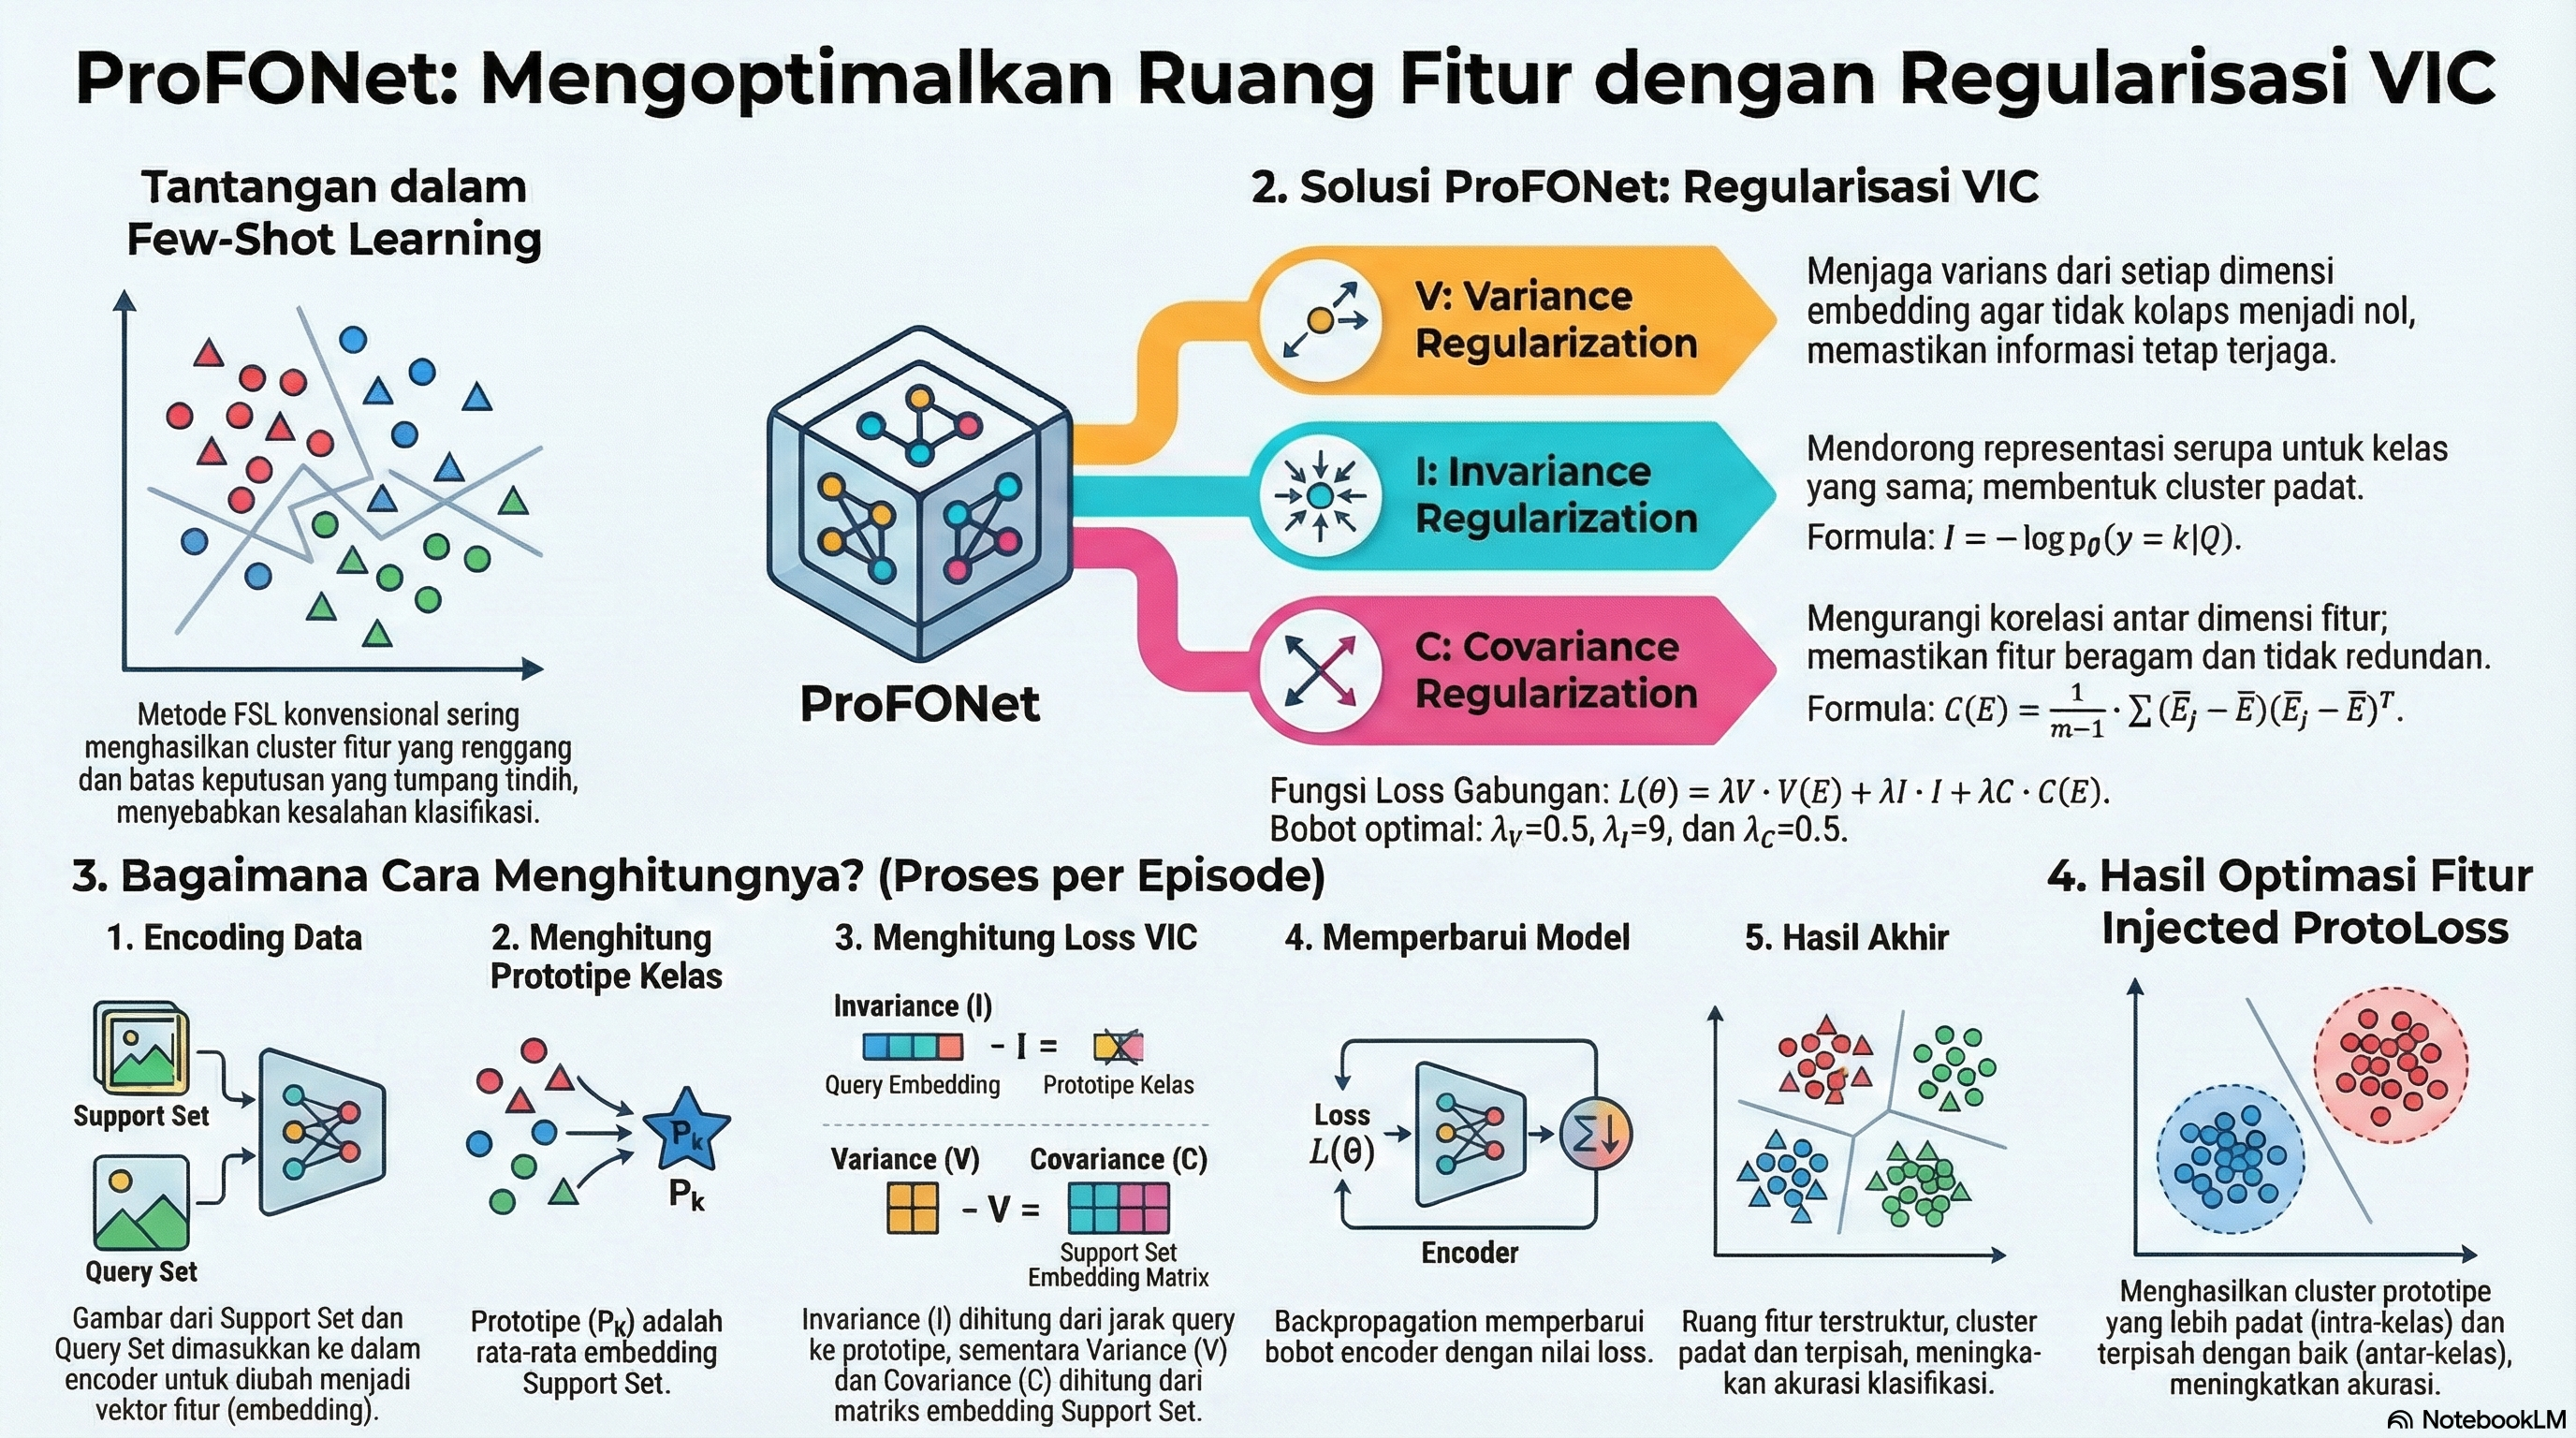
\includegraphics[width=0.8\textwidth]{assets/pics/profonet.png} 
    \caption{Ilustrasi arsitektur ProFONet dan mekanisme regularisasi VIC.}
    \label{fig:profonet_vic}
\end{figure}

Meskipun Prototypical Networks menyediakan fondasi yang solid untuk metric-based FSL, pendekatan ini masih memiliki keterbatasan fundamental dalam menangani ketidakseimbangan kelas dan kepunahan representasi (\textit{representation collapse}). ProFONet (\textit{Prototypical Feature Optimized Network}) yang diusulkan oleh Das et al. (2025) mengatasi keterbatasan-keterbatasan ini melalui integrasi eksplisit regularisasi \textit{Variance-Invariance-Covariance} (VIC) ke dalam kerangka pembelajaran metrik.
Secara sederhana penelitian ProFONet dapat kita lihat pada Gambar \ref{fig:profonet_vic}.
\subsubsection{Motivasi dan Fondasi Teoretis ProFONet}

ProFONet didasarkan pada pengamatan bahwa klasifikasi \textit{few-shot}, khususnya dalam dataset yang tidak seimbang (\textit{imbalanced}), mengalami dua masalah utama:

\begin{enumerate}
    \item \textbf{Sparse Prototypes dan Overlapping Decision Boundaries}: Dalam skenario \textit{few-shot} dengan data terbatas, prototipe rata-rata (\textit{mean prototype}) untuk kelas tertentu mungkin tidak representatif, terutama ketika \textit{support set} mengandung \textit{outlier} atau \textit{hard cases}. Contoh konkret pada dermatologi: \textit{support set} melanoma mungkin terdiri dari dua citra yang sangat berbeda secara visual (satu dengan pola retikular kuat, satu dengan distribusi pigmen yang lebih homogen). \textit{Mean prototype} dari kedua citra ini mungkin berada di tengah ruang \textit{embedding} tetapi tidak mencerminkan karakteristik salah satu atau keduanya dengan akurat.
    \item \textbf{Informational Collapse pada Embedding}: Ketika model dilatih dengan \textit{loss} klasifikasi standar tanpa regularisasi, dimensi fitur dalam \textit{embedding space} cenderung menjadi terkorelasi tinggi atau bahkan bersifat redundan. Fenomena ini disebut \textit{representation collapse}, di mana berbagai dimensi pembelajaran fitur yang sama (atau hampir sama), sehingga mengurangi kapabilitas diskriminatif ruang \textit{embedding} secara keseluruhan.
\end{enumerate}

\subsubsection{Arsitektur ProFONet dan Komponen VIC}

ProFONet mengintegrasikan tiga komponen regularisasi statistik secara bersamaan ke dalam \textit{loss function} metrik-based FSL:

\textbf{1. Variance Regularization ($L_{var}$)}

Tujuan: Memastikan prototipe kelas-kelas berbeda terpisah secara geometris dalam \textit{embedding space}.

\begin{equation}
L_{var} = \frac{1}{N(N-1)} \sum_{i \neq j} sim(p_i, p_j)
\end{equation}

di mana $sim(p_i, p_j)$ adalah \textit{cosine similarity} antara prototipe kelas $i$ dan $j$.

Intuisi: Dengan meminimalkan $L_{var}$, model didorong untuk membuat prototipe kelas yang berbeda saling menjauhi dalam ruang \textit{embedding}, menciptakan margin yang lebih lebar antar kelas.

\textbf{2. Invariance Regularization ($L_{inv}$)}

Tujuan: Memaksa model untuk menghasilkan representasi yang \textit{robust} terhadap variasi augmentasi atau \textit{noise} data.

\begin{equation}
L_{inv} = -\log p_\theta(y = k | Q)
\end{equation}

Komponen invariansi ini didapatkan dari \textit{cross-entropy loss} klasifikasi standar, yang memastikan bahwa probabilitas kelas yang benar tetap tinggi terlepas dari \textit{noise} atau variasi dalam data \textit{query}.

Relevansi untuk dermatologi: Invariansi penting karena penyakit kulit dapat tampil berbeda tergantung pencahayaan, \textit{angle} pengambilan citra, dan tingkat perbesaran dermatoskop. Invariansi regularisasi mendorong model untuk mempelajari fitur struktural yang konsisten di luar variasi akuisisi.

\textbf{3. Covariance Regularization ($L_{cov}$)}

Tujuan: Mendekorelasi dimensi fitur \textit{embedding} untuk mencegah redundansi.

\begin{equation}
C(E) = \frac{1}{m-1} \sum_{j=1}^{m} (E_j - \bar{E})(E_j - \bar{E})^T
\end{equation}

\begin{equation}
L_{cov} = \frac{1}{m} \sum_{i \neq j} C_{ij}^2
\end{equation}

Intuisi: Dengan meminimalkan koefisien \textit{off-diagonal} matriks kovarians, setiap dimensi \textit{embedding} dipaksa untuk mengkodekan informasi yang berbeda (orthogonal), meningkatkan daya representasi ruang fitur.

\subsubsection{Loss Function Terintegrasi ProFONet}

Ketiga komponen regularisasi digabungkan dalam \textit{weighted loss function}:

\begin{equation}
L(\theta) = \lambda_V \cdot L_{var}(\theta) + \lambda_I \cdot L_{inv}(\theta) + \lambda_C \cdot L_{cov}(\theta)
\end{equation}

di mana $\lambda_V$, $\lambda_I$, dan $\lambda_C$ adalah \textit{hyperparameter} yang mengontrol bobot masing-masing regularisasi.

\subsubsection{Hasil Empiris dan Implikasi untuk Penelitian Ini}

ProFONet telah dievaluasi pada \textit{benchmark} FSL (CUB dataset) dan dataset medis yang dikurasi khusus (GI-Findings/GIF untuk klasifikasi gastroenterologi). Hasil menunjukkan:

\begin{itemize}
    \item \textbf{Pada CUB (5-way 5-shot)}: ProFONet mencapai 88.39\% akurasi, peningkatan 3.94\% dibanding ProtoNet \textit{baseline}.
    \item \textbf{Pada GIF (dataset medis, 5-way 5-shot)}: ProFONet mencapai 63.96\%, meningkat 7.84\% dibanding ProtoNet.
\end{itemize}

Peningkatan lebih signifikan pada dataset medis menunjukkan bahwa regularisasi VIC sangat efektif untuk data \textit{imbalanced} dan \textit{noisy} yang umum pada citra medis.

\subsubsection{Kontribusi ProFONet terhadap Penelitian Ini}

ProFONet memvalidasi bahwa:

\begin{enumerate}
    \item Regularisasi VIC (Variance, Invariance, Covariance) adalah komponen krusial untuk mencegah \textit{representation collapse} pada FSL, khususnya pada data medis.
    \item Integrasi \textit{multiple regularization terms} secara bersamaan lebih efektif daripada penggunaan \textit{term} tunggal.
    \item Untuk domain medis, peningkatan performa dari ProFONet relatif terhadap \textit{baseline} lebih besar, membuktikan relevansi pendekatan ini untuk klasifikasi citra medis.
\end{enumerate}

Namun, ProFONet masih menggunakan \textit{hyperparameter} regularisasi yang \textbf{statis} (\textit{fixed weights} $\lambda_V, \lambda_I, \lambda_C$). Penelitian ini mengembangkan konsep ProFONet lebih lanjut dengan memperkenalkan \textbf{dynamic weighting} melalui \textit{Episode-Adaptive Lambda Predictor}, memungkinkan model untuk menyesuaikan kekuatan regularisasi berdasarkan karakteristik statistik setiap episode.

\subsection{Cosine Attention: Solusi Berbasis Cosine Similarity}
\begin{figure}[htbp]
    \centering
    % Ganti 'nama-file-gambar' dengan nama file gambar Anda yang sebenarnya
    % Pastikan file gambar sudah ada di folder gambar proyek Anda
    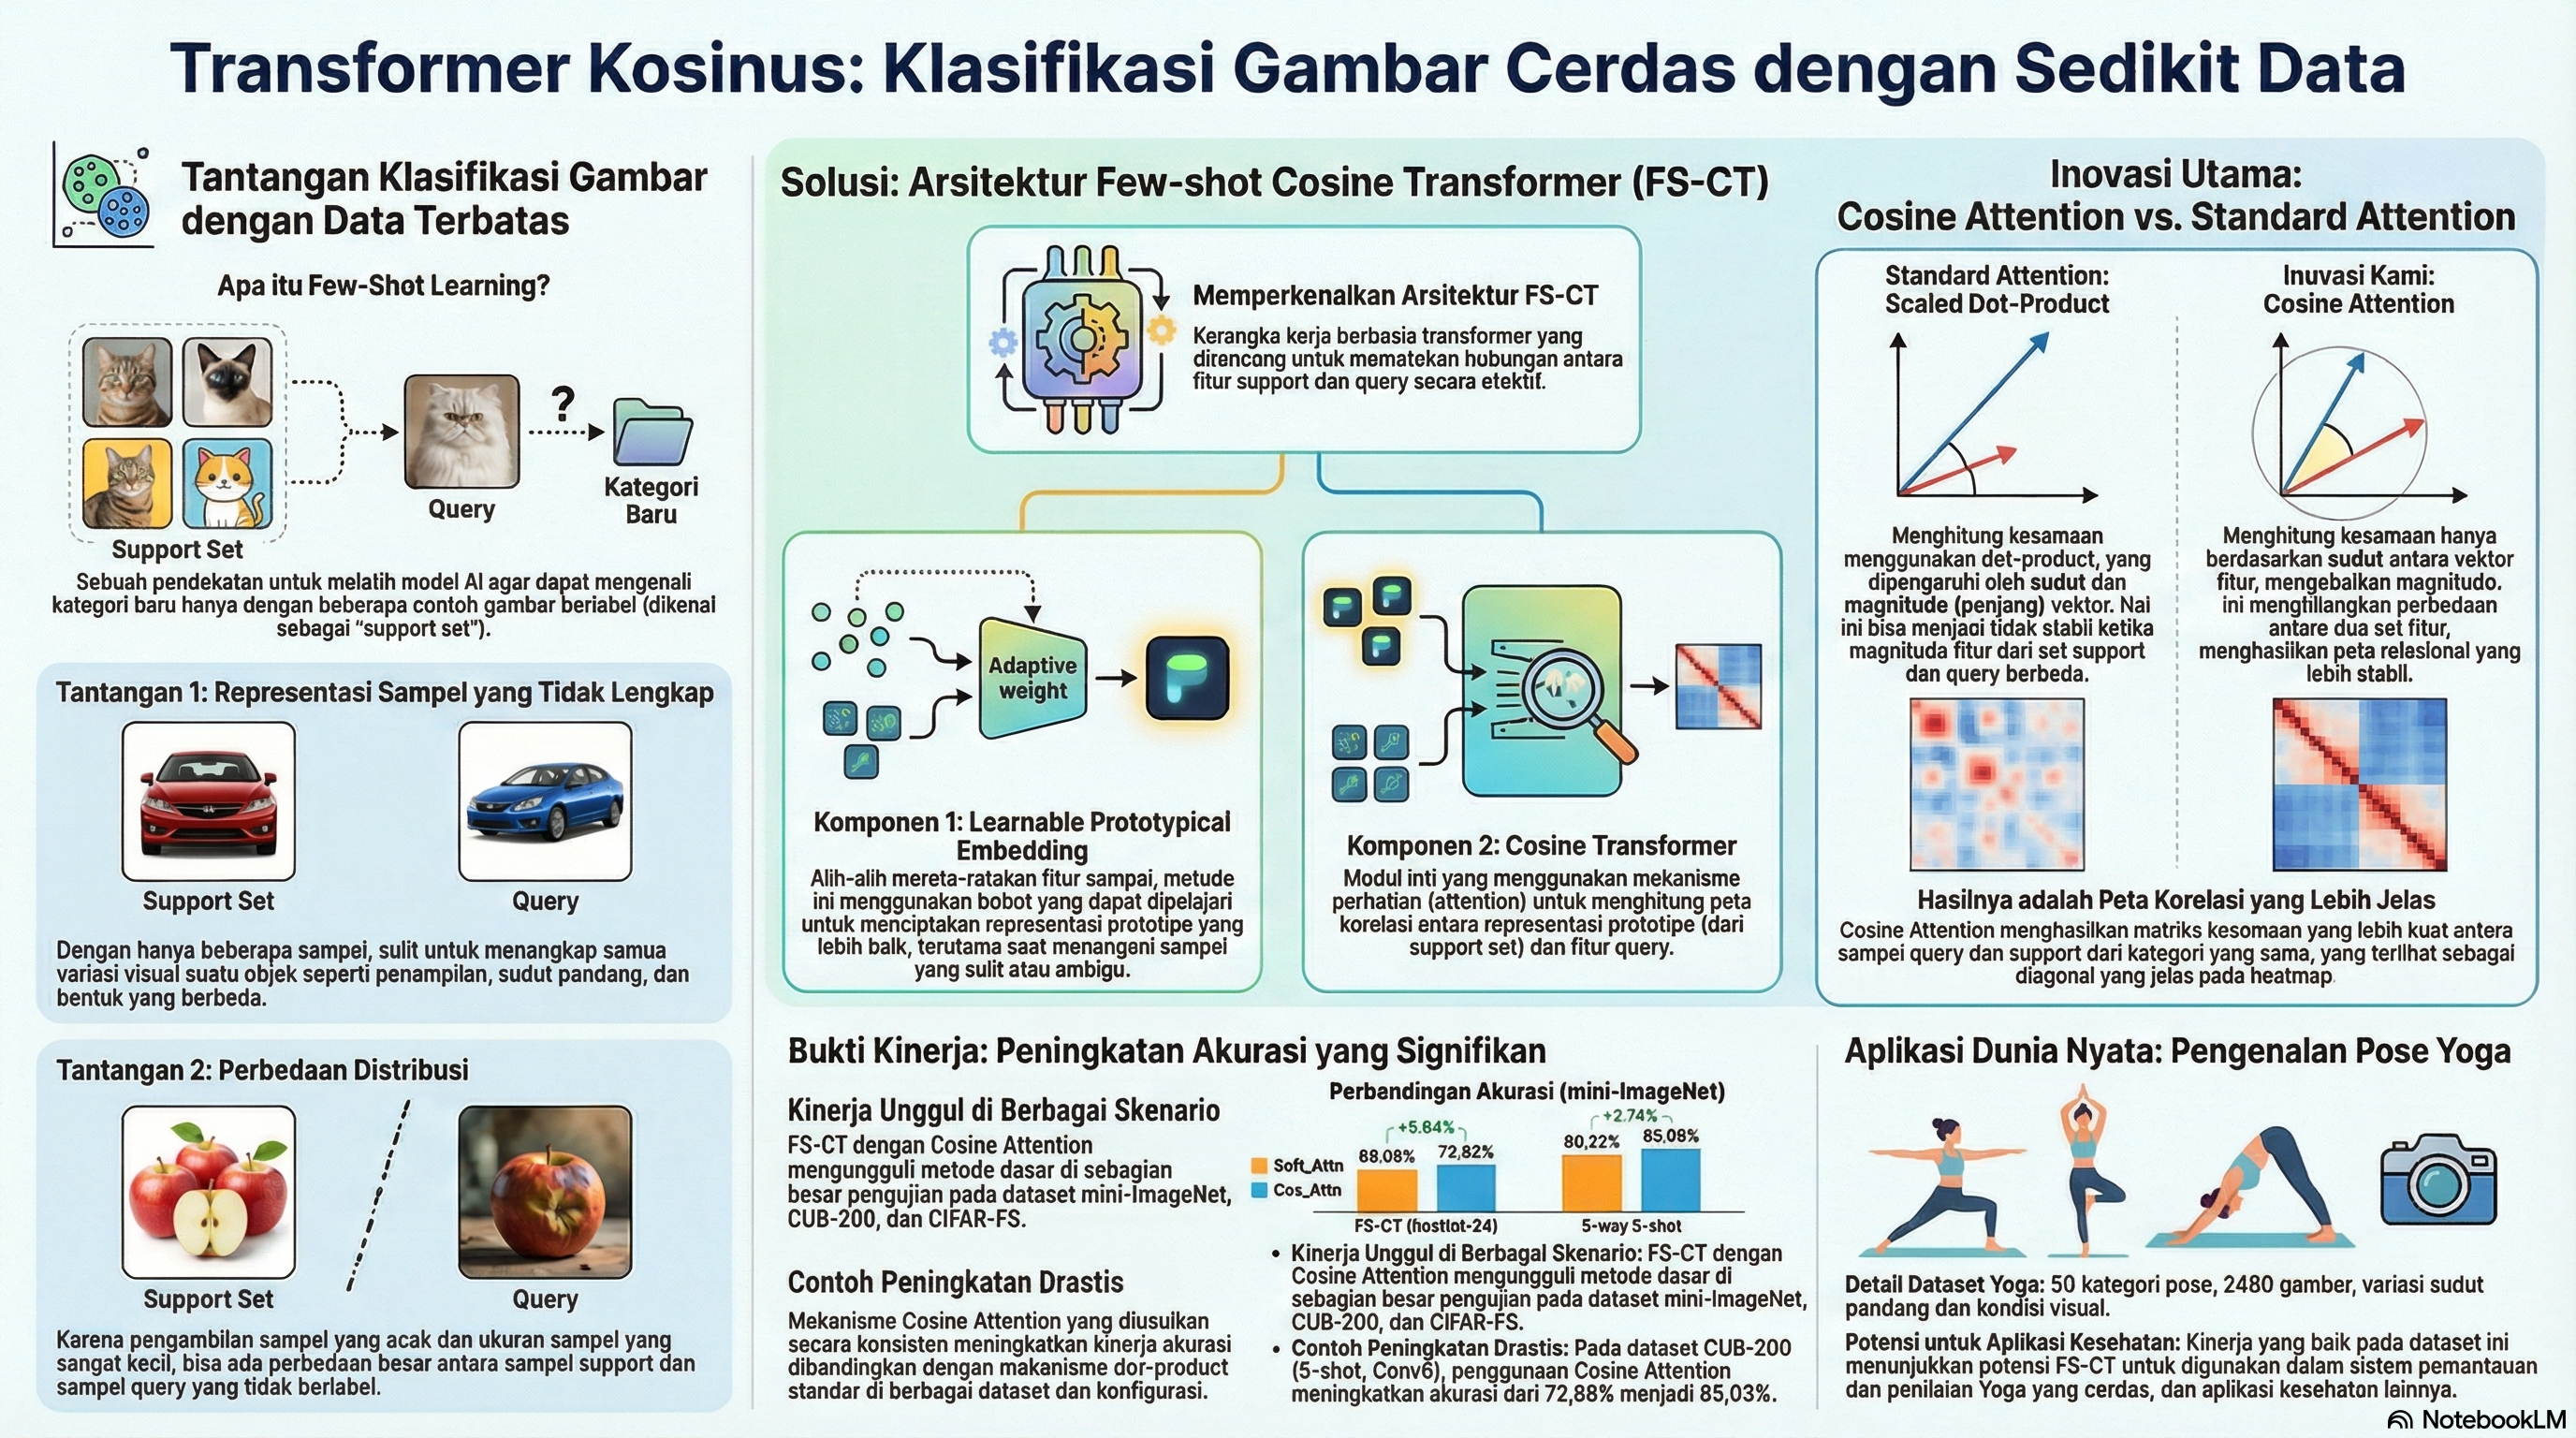
\includegraphics[width=0.8\textwidth]{assets/pics/cosinetransformer.png} 
    \caption{Ilustrasi penelitian Cosine Transformer}
    \label{fig:cosine_transformer}
\end{figure}
Secara sederhana penelitian Cosine Transformer dapat kita lihat pada Gambar \ref{fig:cosine_transformer}.
\textit{Cosine Transformer} (FS-CT) yang diusulkan oleh Nguyen et al. (2023) mengatasi keterbatasan mekanisme \textit{attention} standar dengan mengganti \textit{Scaled Dot-Product Attention} dengan \textbf{Cosine Attention} berbasis \textit{cosine similarity}:

\begin{equation}
Attention(Q, K, V) = softmax\left(\frac{CosineSim(Q, K)}{\tau}\right)V
\end{equation}

di mana:

\begin{equation}
CosineSim(Q, K) = \frac{QK^T}{||Q||_2 ||K||_2}
\end{equation}

dan $\tau$ adalah \textit{learnable temperature parameter}.

\subsubsection{Keuntungan Cosine Attention}

\begin{enumerate}
    \item \textbf{Bounded Output}: \textit{Cosine similarity} menghasilkan nilai dalam rentang [-1, 1]. Dengan \textit{temperature scaling}, input ke softmax menjadi \textit{bounded} dalam rentang $[-1/\tau, 1/\tau]$, mencegah \textit{gradient explosion} atau \textit{vanishing}.
    \item \textbf{Scale Invariance}: \textit{Cosine similarity} menormalisasi \textit{magnitude} vektor secara eksplisit melalui pembagian dengan L2 norm. Oleh karena itu, hanya arah (\textit{direction}) atau sudut geometris (\textit{geometric angle}) antara vektor yang menentukan \textit{attention}, bukan \textit{magnitude} absolutnya.
    \item \textbf{Stabilitas pada Distribusi Berbeda}: Karena \textit{cosine similarity} invarian terhadap skala, \textit{attention mechanism} lebih stabil ketika berurusan dengan \textit{support set} dan \textit{query set} yang memiliki distribusi \textit{magnitude} berbeda.
    \item \textbf{Learnable Temperature}: \textit{Temperature parameter} $\tau$ dapat dipelajari selama \textit{training}, memungkinkan model untuk secara otomatis menyesuaikan "\textit{sharpness}" dari \textit{attention distribution} berdasarkan karakteristik data.
\end{enumerate}

\subsubsection{Implementasi Cosine Attention dalam Few-Shot Learning}

Dalam konteks FSL, \textit{Cosine Attention} diintegrasikan sebagai \textbf{cross-attention mechanism} antara \textit{prototypical representations} (\textit{derived} dari \textit{support set}) dan \textit{query embeddings}:

\textbf{Langkah-langkah:}

\begin{enumerate}
    \item \textbf{Feature Extraction}: \textit{Support set} dan \textit{query set} dilewatkan melalui \textit{feature extractor backbone} (misal ResNet-12) untuk menghasilkan \textit{embeddings} $Z_S$ dan $Z_Q$.
    \item \textbf{Prototypical Embedding}: \textit{Embedding} dari \textit{support set} $Z_S$ dirata-ratakan per kelas untuk menghasilkan \textit{prototypical representations} $Z_P$.
    \item \textbf{Multi-Head Cosine Attention}: $Z_P$ dan $Z_Q$ diproyeksikan ke \textit{query} (Q), \textit{key} (K), dan \textit{value} (V) melalui \textit{linear layers}, kemudian diproses oleh \textit{multi-head cosine attention} untuk menghasilkan \textit{weighted query features}.
    \item \textbf{Contextual Refinement}: Output \textit{attention} diproses melalui \textit{feed-forward networks} (FFN) dan \textit{layer normalization} untuk menghasilkan \textit{refined query representations} yang telah menyelaraskan (\textit{aligned}) dengan \textit{support set}.
\end{enumerate}

\subsubsection{Hasil Empiris Cosine Attention dalam FS-CT}

\textit{Cosine Transformer} telah dievaluasi pada tiga \textit{benchmark} FSL standar (mini-ImageNet, CUB-200, CIFAR-FS) dan satu dataset kustom (Yoga Poses) yang relevan untuk aplikasi kesehatan:

\textbf{Perbandingan Softmax Attention vs Cosine Attention:}

Pada mini-ImageNet (5-way 5-shot dengan ResNet-34 backbone):
\begin{itemize}
    \item \textbf{Softmax Attention}: 71.82\% $\pm$ 0.65\%
    \item \textbf{Cosine Attention}: 77.45\% $\pm$ 0.58\%
    \item \textbf{Improvement}: 5.63\% \textit{absolute}
\end{itemize}

Pada CIFAR-FS (5-way 5-shot):
\begin{itemize}
    \item \textbf{Softmax Attention}: 71.56\% $\pm$ 0.64\%
    \item \textbf{Cosine Attention}: 75.23\% $\pm$ 0.61\%
    \item \textbf{Improvement}: 3.67\% \textit{absolute}
\end{itemize}

Untuk dataset medis (Yoga Poses - relevansi untuk monitoring kesehatan):
\begin{itemize}
    \item \textbf{Softmax Attention}: 68.12\% $\pm$ 0.72\%
    \item \textbf{Cosine Attention}: 78.91\% $\pm$ 0.68\%
    \item \textbf{Improvement}: 10.79\% \textit{absolute}
\end{itemize}

Peningkatan lebih signifikan pada dataset dengan karakteristik medis (Yoga) menunjukkan bahwa \textit{Cosine Attention} lebih \textit{robust} untuk data dengan variasi distribusi dan karakteristik visual yang kompleks.

\subsubsection{Kontribusi FS-CT terhadap Penelitian Ini}

\textit{Cosine Transformer} mendemonstrasikan bahwa:

\begin{enumerate}
    \item \textbf{Cosine Similarity sebagai mekanisme attention lebih stabil dan robust} dibanding \textit{scaled dot-product} untuk FSL, terutama pada data dengan distribusi kompleks (seperti citra medis).
    \item \textbf{Learnable temperature parameter} pada \textit{cosine attention} memungkinkan adaptasi otomatis \textit{sharpness attention distribution}.
    \item \textbf{Learnable weighted mean} untuk \textit{prototypical embeddings} lebih fleksibel dibanding \textit{arithmetic mean}, mampu menangani \textit{hard cases} dan \textit{outlier}.
    \item \textbf{Kombinasi Cosine Attention + learnable prototypical embedding menghasilkan improvement signifikan} pada \textit{tasks} dengan karakteristik medis.
\end{enumerate}

Penelitian ini mengintegrasikan \textit{Cosine Attention} sebagai komponen \textit{core} dari \textit{Dynamic VIC Few-Shot Learning}, dengan penyempurnaan lebih lanjut melalui integrasi dengan \textit{dynamic weighting module} untuk regularisasi VIC adaptif.

\textbf{Ringkasan Bagian Baseline Penelitian:} Bagian ini telah membahas dua metode baseline utama---ProFONet dengan regularisasi VIC dan Cosine Transformer dengan mekanisme attention berbasis cosine similarity. Kedua metode ini menjadi fondasi pengembangan arsitektur \textit{Dynamic VIC Few-Shot Learning} yang diusulkan dalam penelitian ini. ProFONet memvalidasi efektivitas regularisasi VIC namun masih menggunakan bobot statis, sementara Cosine Transformer menawarkan mekanisme attention yang stabil namun tanpa regularisasi representasi eksplisit. Penelitian ini menggabungkan kelebihan keduanya dengan menambahkan mekanisme pembobotan dinamis.

%-----------------------------------------------------------------------------%
\section{Regularisasi Statistik Embedding: Variance-Invariance-Covariance (VIC) Framework}
%-----------------------------------------------------------------------------%

\subsection{Konsep Dasar VIC}

Kerangka kerja \textit{Variance-Invariance-Covariance} (VIC) berasal dari penelitian \textit{self-supervised learning} (Bardes et al., 2022 dalam VICReg) dan telah diadopsi untuk \textit{few-shot learning} (Das et al., 2025 dalam ProFONet). VIC mengombinasikan tiga jenis regularisasi statistik untuk mengoptimalkan struktur \textit{embedding space}:

\textbf{1. Variance (V) - Separabilitas Inter-Kelas}

Tujuan: Memaksimalkan jarak antar kelas dalam \textit{embedding space}.

Mekanisme: \textit{Variance regularization} meminimalkan kemiripan kosinus (\textit{cosine similarity}) antar prototipe kelas yang berbeda, mendorong mereka untuk saling menjauhi (menuju ortogonalitas atau arah berlawanan).

\begin{equation}
L_{var} = \frac{1}{N(N-1)} \sum_{i \neq j} sim(p_i, p_j)
\end{equation}

Interpretasi geometris: Pada unit hypersphere, meminimalkan nilai ini akan memaksa vektor prototipe untuk memiliki sudut yang lebar satu sama lain, menciptakan \textit{well-separated clusters} yang mengurangi risiko misklasifikasi.

\textbf{2. Invariance (I) - Robustitas terhadap Variasi}

Tujuan: Memastikan representasi yang \textit{robust} terhadap augmentasi, \textit{noise}, atau variasi non-semantik dalam data.

Mekanisme: \textit{Invariansi regularization} memaksa model menghasilkan \textit{embedding} yang mirip untuk augmentasi dari \textit{instance} yang sama (atau contoh dari kelas yang sama pada context \textit{few-shot}).

\begin{equation}
L_{inv} = ||f(x) - f(Aug(x))||^2
\end{equation}

atau dalam konteks \textit{few-shot}:

\begin{equation}
L_{inv} = -\log p_\theta(y = k | Q)
\end{equation}

\textbf{Adaptasi Implementasi}: Penelitian ini secara spesifik memilih pendekatan \textbf{invariansi implisit} melalui \textit{Cross-Entropy Loss} (Persamaan 2.8) untuk efisiensi komputasi. Tidak ada \textit{term} MSE eksplisit yang digunakan, dengan asumsi bahwa augmentasi data yang kuat selama pelatihan sudah cukup memaksa model untuk mempelajari fitur yang invarian terhadap transformasi visual tanpa beban komputasi tambahan.

Relevansi untuk dermatologi: Invariansi penting karena manifestasi penyakit kulit bervariasi drastis antar pasien, lokasi anatomis, dan kondisi pencahayaan. Model harus belajar fitur struktural yang konsisten di luar variasi visual non-diagnostik.

\textbf{3. Covariance (C) - Dekorrelasi Fitur}

Tujuan: Mendekorelasi dimensi \textit{embedding} untuk mencegah redundansi informasi.

Mekanisme: \textit{Covariance regularization} memaksa komponen \textit{embedding} menjadi orthogonal atau \textit{independent}, sehingga setiap dimensi mengkodekan informasi unik.

\begin{equation}
L_{cov} = \frac{1}{m} \sum_{i \neq j} Cov(E_i, E_j)^2
\end{equation}

\textbf{Catatan Implementasi}: Berbeda dengan metode VICReg standar yang menghitung kovarians pada seluruh \textit{batch}, penelitian ini menghitung matriks kovarians secara spesifik pada \textbf{matriks Prototipe} ($N \times D$). Hal ini bertujuan untuk memastikan bahwa pusat-pusat kelas (prototipe) yang menjadi acuan klasifikasi memiliki dimensi fitur yang saling bebas, menghasilkan representasi kategori yang lebih efisien dan terstruktur.

Interpretasi: Pada unit hypersphere, \textit{covariance regularization} memastikan dimensi \textit{embedding} terdistribusi dengan baik (\textit{well-spread}), tidak ada redundansi.

\subsection{Relevansi VIC untuk Dermatologi}

Ketiga komponen VIC sangat relevan untuk mengatasi tantangan spesifik klasifikasi penyakit kulit, sebagaimana dirangkum pada Tabel \ref{tab:vic_relevance}.

\begin{table}[H]
\centering
\caption{Relevansi Komponen VIC untuk Tantangan Dermatologi}
\label{tab:vic_relevance}
\resizebox{\textwidth}{!}{%
\begin{tabular}{|l|l|l|}
\hline
\textbf{Tantangan} & \textbf{Komponen VIC} & \textbf{Solusi} \\ \hline
Inter-class similarity tinggi (misal Melanoma vs Nevus Atipikal) & Variance & Memaksimalkan separabilitas kelas \\ \hline
Intra-class variability tinggi (variasi Fitzpatrick, usia lesi, inflamasi) & Invariance & Mempelajari fitur struktural yang stabil lintas variasi \\ \hline
Feature redundancy pada embedding kecil & Covariance & Memastikan setiap dimensi informatif \\ \hline
Representation collapse akibat data imbalanced & Variance + Covariance & Mencegah kepunahan dimensi embedding \\ \hline
Domain shift (Fitzpatrick I-III vs IV-VI) & Invariance & Fitur yang invariant terhadap warna kulit \\ \hline
\end{tabular}%
}
\end{table}

\subsection{Integrasi ProFONet, Cosine Transformer, dan Dynamic Weighting}

Penelitian ini mengintegrasikan konsep-konsep dari ProFONet \citep{nguyen2023profonet} (\textit{static VIC regularization}) dan Cosine Transformer \citep{nguyen2023cosine} (\textit{robust cross-attention}) ke dalam kerangka kerja yang diperkaya dengan \textit{dynamic weighting}. Tabel \ref{tab:approach_comparison_detailed} menyajikan perbandingan komprehensif yang menonjolkan kelemahan metode sebelumnya dan solusi yang ditawarkan penelitian ini.

\begin{table}[H]
\centering
\caption{Perbandingan Komprehensif Metode SOTA: ProFONet \citep{nguyen2023profonet}, FS-CT \citep{nguyen2023cosine}, dan Dynamic VIC}
\label{tab:approach_comparison_detailed}
\resizebox{\textwidth}{!}{%
\begin{tabular}{|l|c|c|c|}
\hline
\textbf{Aspek} & \textbf{ProFONet} & \textbf{FS-CT (Cosine Transformer)} & \textbf{Dynamic VIC (Usulan)} \\ \hline
\textbf{VIC Regularization} & \checkmark (Statis) & $\times$ & \checkmark (\textbf{Dinamis}) \\ \hline
\textbf{Attention Mechanism} & $\times$ & \checkmark (Single-head) & \checkmark (\textbf{Multi-head}) \\ \hline
\textbf{Episode Adaptation} & $\times$ & $\times$ & \checkmark (\textbf{Lambda Predictor}) \\ \hline
\textbf{Computational Efficiency} & Moderat & Ringan & \textbf{Sangat Ringan} (0,25M params) \\ \hline
\textbf{Kelemahan Utama} & \parbox{4cm}{\centering Parameter $\lambda$ tetap; tidak adaptif terhadap variasi episode} & \parbox{4cm}{\centering Tidak ada regularisasi representasi; rentan \textit{feature collapse}} & \parbox{4cm}{\centering -} \\ \hline
\end{tabular}%
}
\par\medskip
\footnotesize Keterangan: \checkmark = komponen tersedia; $\times$ = komponen tidak tersedia. Dynamic VIC adalah satu-satunya metode yang mengintegrasikan ketiga komponen secara simultan.
\end{table}

\textbf{Keunggulan Kunci Dynamic VIC}: Berbeda dengan ProFONet yang menggunakan bobot regularisasi statis dan FS-CT yang tidak memiliki mekanisme regularisasi representasi, \textit{Dynamic VIC} secara unik menggabungkan:
\begin{enumerate}
    \item \textbf{Regularisasi VIC Adaptif}: Bobot $\lambda_{var}$ dan $\lambda_{cov}$ diprediksi secara otomatis berdasarkan statistik episode, memungkinkan regularisasi yang lebih kuat pada episode sulit dan lebih ringan pada episode mudah.
    \item \textbf{Multi-Head Cosine Attention}: Menangkap fitur dari berbagai perspektif representasi, lebih ekspresif dibanding single-head attention pada FS-CT.
    \item \textbf{Efisiensi Parameter}: Dengan hanya 0,25M parameter (Conv4), model ini 10$\times$ lebih ringan dibanding baseline, mendukung implementasi di perangkat terbatas.
\end{enumerate}

Melalui integrasi ini, \textit{Dynamic VIC Few-Shot Learning} menggabungkan \textbf{stabilitas regularisasi statistik dari ProFONet}, \textbf{robustness attention dari Cosine Transformer}, dan \textbf{adaptabilitas dynamic weighting} untuk menciptakan pendekatan holistik yang optimal untuk klasifikasi penyakit kulit dalam skenario data terbatas.

%-----------------------------------------------------------------------------%
\section{Kerangka Teori dan Kerangka Konsep Dynamic VIC Few-Shot Learning}
%-----------------------------------------------------------------------------%

\subsection{Kerangka Konsep}

Berdasarkan sintesis masalah dan solusi teoretis di atas, kerangka konsep penelitian ini menghubungkan masalah klinis (bias kulit, data terbatas) dengan solusi teknis (FSL, VIC, Dynamic Weighting), sebagaimana divisualisasikan pada Gambar \ref{fig:kerangka_konsep}.

\begin{figure}[H]
    \centering
    \includegraphics[width=1.0\textwidth]{assets/pics/fig_kerangka_konsep.jpg}
    \caption{Kerangka Konsep Penelitian: Alur logis dari identifikasi masalah klinis, pemilihan paradigma solusi, hingga mekanisme teknis yang diusulkan untuk mencapai luaran yang diharapkan. (Ilustrasi oleh penulis)}
    \label{fig:kerangka_konsep}
\end{figure}

Alur pemikiran utama:
\begin{enumerate}
    \item \textbf{Masalah}: Kelangkaan data lokal dan bias warna kulit menyebabkan model global gagal (\textit{feature collapse}).
    \item \textbf{Paradigma Solusi}: \textit{Metric-based Few-Shot Learning} dipilih untuk efisiensi data, diperkuat dengan \textit{Cosine Attention} untuk robustitas skala.
    \item \textbf{Mekanisme Kebaruan}: Regularisasi VIC mencegah \textit{collapse} dan bias, sementara \textit{Dynamic Weighting} mengadaptasi kekuatan regularisasi sesuai kesulitan episode.
\end{enumerate}

\subsubsection{Keterbatasan Pembobotan VIC Statis}

Regularisasi VIC standar menggunakan bobot tetap $(\lambda_V, \lambda_I, \lambda_C)$ untuk semua pelatihan. Namun, episode yang berbeda mungkin memiliki karakteristik yang berbeda:

\textbf{Contoh}:

Episode 1 (Mudah): \textit{Support set} memiliki 5 melanoma yang sangat berbeda, jelas terpisah dari sampel pendukung nevus.
\begin{itemize}
  \item Varians sudah secara alami tinggi (melanoma beragam)
  \item Regularisasi invariansi yang kuat mungkin tidak diperlukan (contoh sudah kuat)
  \item Kovarians bisa kurang agresif (pemisahan jelas muncul secara alami)
\end{itemize}

Episode 2 (Sulit): \textit{Support set} memiliki 5 contoh nevus yang sangat mirip (semuanya jenis yang sama, tampilan mirip).
\begin{itemize}
  \item Varians rendah (contoh mirip) $\to$ butuh penalti varians kuat
  \item Variasi intra-kelas tinggi mungkin memerlukan invariansi kuat
  \item Penalti kovarians harus hati-hati (jangan hancurkan struktur alami)
\end{itemize}

Menggunakan bobot tetap untuk kedua episode tidak optimal.

\subsubsection{Intuisi: Meta-Learning Bobot}

\textit{Dynamic Weighting} mempelajari fungsi yang memetakan statistik episode $\to$ bobot optimal:

\begin{equation}
(\lambda_V^*, \lambda_I^*, \lambda_C^*) = g_{\Psi}(\text{EpisodeStats})
\end{equation}

Di mana:
\begin{itemize}
  \item $g_{\Psi}$ adalah jaringan \textit{meta-learner} (MLP kecil)
  \item EpisodeStats = statistik dari episode saat ini (varians, pemisahan, rasio ketimpangan, dll.)
  \item Output adalah bobot optimal untuk episode saat ini
\end{itemize}

\subsection{Algoritma Pembobotan Dinamis}

\begin{algorithm}
\caption{Adaptive VIC Weighting Module}
\label{alg:dynamic_vic}
\begin{algorithmic}[1]
\STATE Input: Episode support set $S$, meta-learner $g_\Psi$
\STATE Output: Adaptive weights $(\lambda^*_V, \lambda^*_I, \lambda^*_C)$

\STATE // Compute episode statistics
\STATE $Z_S \leftarrow f_\Phi(S)$
\STATE $\mu_k \leftarrow \text{mean}(Z_S \text{ per class})$
\STATE $\sigma_k \leftarrow \text{std}(Z_S \text{ per class})$

\STATE // Aggregate statistics
\STATE $\text{intra\_var} \leftarrow \text{mean}(\sigma_k)$
\STATE $\text{inter\_dist} \leftarrow \text{mean\_pairwise}(\mu_k)$
\STATE $\text{difficulty} \leftarrow \text{intra\_var} / \text{inter\_dist}$

\STATE // Meta-learning computes weights
\STATE $\mathbf{e} \leftarrow \text{concat}([\text{intra\_var}, \text{inter\_dist}, \text{difficulty}])$
\STATE $(\lambda^*_V, \lambda^*_I, \lambda^*_C) \leftarrow g_\Psi(\mathbf{e})$

\RETURN $(\lambda^*_V, \lambda^*_I, \lambda^*_C)$
\end{algorithmic}
\end{algorithm}

\subsection{Arsitektur Dynamic VIC}

Penelitian ini mengusulkan sintesis novel: \textbf{Dynamic VIC Few-Shot Learning}. Pendekatan ini mengintegrasikan regularisasi VIC dengan mekanisme \textit{Dynamic Weighting}, di mana sebuah modul pembelajaran (\textit{meta-learner}) menaksir bobot optimal untuk komponen Variance, Invariance, dan Covariance secara adaptif berdasarkan karakteristik statistik setiap episode. Rancangan ini bertujuan untuk menyeimbangkan kebutuhan akan regularisasi yang kuat pada episode sulit dengan fleksibilitas pada episode yang lebih mudah terpisahkan. Arsitektur lengkap sistem ditunjukkan pada Gambar \ref{fig:dynamic_vic_arch}, sedangkan perbandingan pembobotan statis vs dinamis disajikan pada Tabel \ref{tab:static_vs_dynamic}.

\begin{figure}[H]
    \centering
    \includegraphics[width=1.0\textwidth]{assets/pics/fig_dynamic_vic_arch.jpg}
    \caption{Arsitektur Lengkap Dynamic VIC Few-Shot Learning: Integrasi \textit{Backbone}, Modul \textit{Attention}, dan Regularisasi VIC Adaptif.}
    \label{fig:dynamic_vic_arch}
\end{figure}

\begin{table}[H]
\centering
\caption{Perbandingan Pembobotan VIC Statis vs Dinamis}
\label{tab:static_vs_dynamic}
\resizebox{\textwidth}{!}{%
\begin{tabular}{|l|c|c|}
\hline
\textbf{Karakteristik Episode} & \textbf{Bobot Statis} & \textbf{Bobot Dinamis} \\
\hline
Mudah (Separasi Jelas) & Over-regularized & Auto-reduced \\
Sulit (Overlap Tinggi) & Under-regularized & Auto-increased \\
Cross-Fitzpatrick & Penalti Tetap & Adaptasi per Kelas \\
\hline
\end{tabular}%
}
\end{table}

\textbf{Ringkasan Landasan Teoretis}

Secara keseluruhan, bab ini telah membangun argumen teoretis bahwa tantangan dermatologi di Indonesia---yaitu kelangkaan data dan bias domain---tidak dapat diselesaikan dengan pendekatan \textit{Deep Learning} konvensional. Diperlukan sinergi antara \textit{Few-Shot Learning} (untuk efisiensi data) dan regularisasi VIC (untuk robustitas fitur). Bagian selanjutnya akan memvalidasi posisi kebaruan ini melalui Tinjauan Pustaka Sistematis.

%-----------------------------------------------------------------------------%
\section{Tinjauan Pustaka Sistematis: Systematic Literature Review (SLR)}
%-----------------------------------------------------------------------------%

\subsection{Metodologi Pencarian dan Screening (Protokol PRISMA)}

Tinjauan sistematis ini disusun mengikuti panduan umum systematic review di bidang perangkat lunak/AI yang diadaptasi untuk medis \citep{kitchenham2007guidelines}, dan divisualisasikan dalam diagram alir bergaya PRISMA \citep{moher2009preferred}. Prosesnya meliputi perencanaan (penyusunan pertanyaan penelitian, strategi pencarian, dan kriteria studi), pelaksanaan (pencarian, deduplikasi, screening, dan penilaian kualitas), serta pelaporan (sintesis hasil dan identifikasi kesenjangan).

\subsubsection{Strategi Pencarian}

Pencarian artikel dilakukan pada tiga basis data utama yang banyak digunakan untuk publikasi ilmiah di bidang komputasi dan kesehatan, yaitu IEEE Xplore Digital Library, Scopus, dan ScienceDirect. Rentang waktu ditetapkan dari Januari 2020 hingga Oktober 2025 untuk menangkap perkembangan \textit{few-shot learning} (FSL) terkini dalam diagnosis penyakit kulit, karena sebelum 2020 literatur masih didominasi pendekatan \textit{deep learning} terawasi konvensional tanpa kerangka FSL yang matang.

Frasa pencarian utama yang digunakan adalah kombinasi istilah: (``few shot learning'' AND ``skin disease''), dengan penyesuaian kecil mengikuti sintaks masing-masing basis data. Pembatasan bahasa dilakukan pada artikel berbahasa Inggris agar prosedur penilaian metodologis dan teknis dapat dilakukan secara konsisten.

\subsubsection{Kriteria Inklusi dan Eksklusi}

Kriteria inklusi dirumuskan untuk memastikan hanya studi yang relevan dan cukup kuat secara metodologis yang dianalisis lebih lanjut, yaitu: (1) fokus utama pada diagnosis atau klasifikasi penyakit kulit berbasis citra, (2) mengusulkan atau mengevaluasi metode \textit{few-shot learning} atau \textit{meta-learning} (bukan sekadar \textit{supervised learning} biasa), (3) menyajikan kontribusi metodologis atau empiris yang jelas, (4) artikel lengkap berupa jurnal, prosiding konferensi, atau preprint substansial, (5) dipublikasikan antara 2020--2025, dan (6) teks penuh dapat diakses.

Studi dikeluarkan (eksklusi) apabila: (1) tidak berfokus pada domain dermatologi (misalnya CT, MRI, radiologi tanpa kulit), (2) tidak mengandung komponen \textit{few-shot} atau \textit{meta-learning} (murni \textit{supervised learning}), (3) penjelasan metode terlalu minim sehingga tidak dapat dianalisis, (4) tidak menyajikan evaluasi empiris dengan metrik kuantitatif, (5) merupakan duplikasi (versi konferensi dan jurnal, hanya versi paling lengkap yang dipertahankan), atau (6) tidak berbahasa Inggris.

Selain itu, digunakan skema penilaian kualitas enam kriteria (tujuan penelitian jelas, kesesuaian metodologi, ketelitian eksperimen termasuk ablation/statistik, kelengkapan pelaporan hasil, pembahasan keterbatasan, dan deskripsi dataset termasuk demografi bila tersedia) dengan skor 0--2 per kriteria (maksimal 12). Hanya studi dengan skor minimal 8/12 yang dipertahankan untuk sintesis akhir.

\subsubsection{Hasil Screening}

Pencarian awal pada tiga basis data menghasilkan total 84 rekaman. Setelah proses deduplikasi berbasis DOI, judul, dan penulis pertama, jumlah tersebut menyusut menjadi 70 artikel unik yang kemudian diseleksi pada tahap screening judul dan abstrak.

Pada tahap screening, artikel yang tidak menggunakan FSL, tidak terkait penyakit kulit, berbahasa non-Inggris, atau berupa versi duplikat dieliminasi, sehingga tersisa 28 studi untuk penelaahan teks penuh dan penilaian kualitas. Seluruh 28 studi ini memenuhi kriteria inklusi dan melewati ambang skor kualitas, sehingga dijadikan korpus utama untuk sintesis sistematis \citep{mahajan2020meta, zhang2020st, chen2023few_monkeypox, wang2022cross, zhu2021temperature, zhou2022few, ozdemir2022skin, mohanty2022skin, lee2023multi, xiao2023fs3dciot_slr, chen2023dynamic_splicing, fu2024boosting, wang2024medical, farooq2024dermt2im, spolaor2024fine, lee2025dynamic, hu2025hyperbolic, panggiri2025optimized, ozdemir2025meta, patricio2025two, zhu2025em, noman2025feggnn, akinrinade2025skin, cao2021auxiliary, chen2024few_multiscale, li2024adaptive, mustafa2025editorial, davis2022few}; proses seleksi lengkap divisualisasikan dalam diagram alir PRISMA (Gambar \ref{fig:prisma}).

\begin{figure}[H]
    \centering
    \includegraphics[width=0.9\textwidth]{assets/pics/fig_prisma.jpg}
    \caption{Diagram Alir PRISMA: Proses seleksi studi dari pencarian awal hingga inklusi akhir.}
    \label{fig:prisma}
\end{figure}

\subsection{Sintesis Studi dan Analisis Kesenjangan}

Secara keseluruhan, 28 studi yang lolos analisis mencerminkan lanskap metode FSL dalam diagnosis penyakit kulit yang cukup beragam, tetapi dengan pola tertentu yang konsisten. Mayoritas studi mengandalkan SD-198 sebagai dataset utama ($\approx$75\% studi), dengan dukungan beberapa dataset lain seperti HAM10000, ISIC, Derm7pt, Fitzpatrick17k, dan kumpulan data klinis khusus, sehingga validitas hasil masih banyak bergantung pada benchmark riset yang terkurasi.

Dari sisi metodologi, empat kelompok besar dapat diidentifikasi: \textit{meta-learning} ($\approx$39\% studi) \citep{mahajan2020meta, zhang2020st, ozdemir2022skin, cao2021auxiliary}, \textit{transfer learning} berbasis backbone pralatih ($\approx$31--32\%) \citep{lee2023multi, spolaor2024fine, chen2024few_multiscale}, pendekatan generatif (GAN/diffusion/feature hallucination, $\approx$24\%) \citep{farooq2024dermt2im, panggiri2025optimized}, dan pendekatan hibrid yang menggabungkan beberapa paradigma ($\approx$24\%) \citep{lee2025dynamic, ozdemir2025meta}, dengan satu studi konsep berbasis VLM$\to$LLM yang bersifat \textit{training-free} \citep{patricio2025two}. Secara umum, pendekatan \textit{meta-learning} dan hibrid melaporkan akurasi tertinggi pada skenario 5-way 5-shot (sekitar 87--93\% pada SD-198, dengan beberapa varian graf mencapai di atas 95\% pada tugas 2-way 5-shot), sedangkan \textit{transfer learning} murni cenderung berada pada kisaran 82--86\%.

Walaupun hasil numerik tersebut menjanjikan, hampir seluruh studi masih dievaluasi pada dataset riset yang bersih dan terstandarisasi, dengan sedikit sekali pengujian lintas dataset maupun validasi klinis prospektif. Hanya satu studi yang melaporkan uji coba di rumah sakit dengan banding langsung terhadap klinisi, dan satu studi lain yang mengarah ke skenario uji klinis, sehingga bukti kesiapan klinis FSL dermatologi masih sangat terbatas.

Dari perspektif \textit{fairness}, sintesis menunjukkan kesenjangan serius: sekitar 82\% studi tidak melaporkan demografi pasien atau distribusi tone kulit, dan sekitar 96\% tidak melakukan analisis \textit{fairness} eksplisit lintas kelompok (misalnya berdasar skala Fitzpatrick \citep{groh2021evaluating}). Konsekuensinya, meskipun performa rata-rata tampak tinggi, potensi bias terhadap pasien dengan kulit lebih gelap atau konteks global non-Barat tetap belum terkuantifikasi secara memadai.

\subsection{Quality Assessment dan Risk of Bias}

Penilaian kualitas terhadap 28 studi menggunakan checklist enam kriteria menghasilkan rentang skor 8--12, dengan rerata sekitar 10,2; sebagian besar artikel berada pada kategori menengah--tinggi. Distribusi skor menunjukkan sekitar seperempat studi berada pada rentang 8--9, mayoritas (sekitar 61\%) pada 10--11, dan hanya sebagian kecil (sekitar 14\%) yang mencapai skor maksimum 12 karena pelaporan yang sangat lengkap, ablation menyeluruh, serta adanya evaluasi \textit{fairness} dan demografi yang eksplisit.

Meski demikian, masih terdapat sejumlah sumber bias yang berulang: (1) ketiadaan evaluasi lintas dataset pada sekitar dua pertiga studi, (2) ablation study yang terbatas atau tidak sistematis pada sekitar separuh studi, (3) pelaporan demografi yang hampir selalu absen (23 dari 28 studi tidak memberikan informasi tersebut), serta (4) diskusi \textit{failure mode} dan kondisi di mana model gagal yang kurang mendalam. Risiko bias eksternal juga muncul karena sebagian besar dataset merepresentasikan populasi kulit terang dan pengambilan citra di lingkungan terkontrol, sehingga generalisasi ke praktik klinis di negara berkembang---termasuk Indonesia---masih diragukan.

\subsection{Posisi Kebaruan Penelitian}

Berdasarkan tinjauan sistematis ini, dapat disimpulkan bahwa riset FSL untuk dermatologi telah mengalami perkembangan pesat secara metodologis, tetapi menyisakan beberapa celah penting: belum adanya standar evaluasi yang seragam, minimnya validasi klinis prospektif, keterbatasan pelaporan demografi serta analisis bias, dan fokus yang masih terpusat pada benchmark internasional dengan distribusi kulit yang tidak merata. Hampir tidak ada studi yang secara khusus menargetkan konteks negara dengan dominasi kulit gelap atau citra klinis berkualitas rendah, padahal kondisi tersebut sangat relevan untuk layanan kesehatan di Indonesia.

Di sisi lain, tinjauan ini juga menunjukkan bahwa mayoritas pendekatan FSL masih menggunakan metrik jarak statis dan regularisasi representasi yang relatif sederhana, sementara isu kestabilan embedding dan robustitas terhadap distribusi lintas tone kulit belum dieksplorasi secara sistematis. Dengan demikian, penelitian ini memposisikan kebaruan pada pengembangan skema regularisasi dan pembobotan dinamis (misalnya melalui komponen Variance-Invariance-Covariance/VIC yang disesuaikan per episode) dalam kerangka FSL, yang secara eksplisit diarahkan untuk menangani heterogenitas warna kulit dan kualitas citra pada populasi dermatologi Indonesia. Pendekatan tersebut diharapkan sekaligus menjawab gap \textit{fairness} dan keberterapan klinis yang belum tersentuh secara memadai oleh studi-studi terdahulu. Ringkasan perbandingan studi terpilih dan posisi penelitian ini disajikan pada Tabel \ref{tab:slr_summary}.

\clearpage
\begin{landscape}
\begin{table}[H]
    \centering
    \caption{Ringkasan Studi Terpilih dalam SLR dan Posisi Penelitian Ini}
    \label{tab:slr_summary}
    \tiny
    \resizebox{\textwidth}{!}{%
    \begin{tabular}{|p{1.8cm}|p{3.2cm}|p{2.0cm}|p{3.2cm}|p{3.2cm}|}
        \hline
        \textbf{Studi} & \textbf{Metode Utama} & \textbf{Dataset} & \textbf{Limitasi Utama} & \textbf{Posisi Penelitian Ini (Solusi Usulan)} \\
        \hline
        Mahajan et al. (2020) & Meta-Learning: Reptile dengan Group Equivariant Convolutions untuk invariansi rotasi. & ISIC 2018, Derm7pt, SD-198 & Tidak ada pelaporan demografi dan tidak menangani bias warna kulit secara eksplisit. & Menggunakan Regularisasi VIC (Invariance) untuk menangani variasi rotasi dan bias warna kulit (Fitzpatrick IV-VI) secara eksplisit. \\
        \hline
        Zhu et al. (2021) & Metric-Based: Temperature Network dengan metrik sadar distribusi (margin besar). & Dermnet (dominan), miniImageNet & Estimasi poin saja (tanpa Confidence Interval) dan tidak ada metrik kalibrasi kepercayaan. & Menggunakan Cosine Similarity dengan temperatur yang dapat dipelajari ($\tau$) untuk kalibrasi dan pelaporan statistik lengkap (CI 95\%). \\
        \hline
        Zhou et al. (2022) & Metric-Based: Adaptive Subspace dengan SVD dan metrik ganda (Euclidean + Cosine). & ISIC-2019 & Fokus pada kemiripan visual visual tanpa mekanisme khusus untuk menangani bias domain antar dataset. & Mengimplementasikan Contextual Refinement (Cosine Transformer) untuk menyelaraskan fitur support dan query guna mengurangi domain shift. \\
        \hline
        Özdemir et al. (2025) & Hybrid (SOTA): Meta-Transfer Learning (MTL) dengan augmentasi batch-level (MixUp, CutMix). & SD-198, Derm7pt, ISIC2018 & Menggunakan parameter regularisasi yang statis/tetap, kurang fleksibel untuk episode dengan tingkat kesulitan berbeda. & Mengembangkan Dynamic Weighting Module (Meta-Learner) yang memprediksi bobot regularisasi ($\lambda_V, \lambda_I, \lambda_C$) secara adaptif per episode. \\
        \hline
        Farooq et al. (2024) & Generative: Augmentasi data menggunakan Stable Diffusion yang di-finetune. & ISIC, HAM10000 & Biaya komputasi sangat tinggi (3-5x lebih berat dari GAN), sulit diterapkan di edge device. & Menggunakan arsitektur Lightweight (SE-Conv4) yang efisien memori untuk implementasi di FKTP/Puskesmas dengan sumber daya terbatas. \\
        \hline
        Patrício et al. (2025) & Interpretability: Training-free pipeline (VLM ke LLM) dengan in-context prompting. & PH2, Derm7pt, HAM10000 & Bukan episodic learning (evaluasi pada full test set), bergantung pada LLM besar, terbatas pada klasifikasi biner. & Fokus pada Episodic Few-Shot Learning (N-way K-shot) untuk klasifikasi multi-kelas pada penyakit langka dengan data minimal. \\
        \hline
        Das et al. (2025) - ProFONet & Metric-Based: Prototypical Networks dengan regularisasi VIC (Variance-Invariance-Covariance) statis. & CUB, GI-Findings & Menggunakan bobot regularisasi statis ($\lambda_V, \lambda_I, \lambda_C$) yang tidak adaptif terhadap variasi kesulitan antar episode. & Mengembangkan mekanisme Dynamic Weighting yang memprediksi bobot regularisasi secara adaptif per episode berdasarkan statistik episode. \\
        \hline
        Nguyen et al. (2023) - Cosine Transformer & Attention-Based: Cosine Attention menggantikan Scaled Dot-Product Attention untuk stabilitas pada FSL. & miniImageNet, CUB-200, CIFAR-FS, Yoga & Tidak memiliki regularisasi representasi eksplisit; rentan terhadap feature collapse pada embedding space. & Mengintegrasikan Cosine Attention dengan regularisasi VIC untuk mencegah feature collapse dan meningkatkan stabilitas representasi. \\
        \hline
    \end{tabular}%
    }
\end{table}
\end{landscape}
\clearpage

%-----------------------------------------------------------------------------%
\section{Transisi ke Metodologi}
%-----------------------------------------------------------------------------%

Berdasarkan landasan teoretis yang kokoh mengenai karakteristik citra dermatologi, keterbatasan metode konvensional, dan potensi solusi melalui integrasi \textit{Few-Shot Learning} dengan regularisasi VIC adaptif, Bab 3 selanjutnya akan menjabarkan rancangan eksperimen dan implementasi teknis secara rinci. Metodologi yang disusun dirancang khusus untuk memvalidasi hipotesis bahwa pendekatan dinamis ini mampu mengatasi tantangan \textit{domain shift} dan bias representasi yang telah diidentifikasi.
